\documentclass[10pt]{ctexart}
\usepackage[ruled,vlined]{algorithm2e}
\usepackage{amssymb}
\usepackage{amsmath}
\usepackage{booktabs}
\usepackage{datetime2}
\usepackage{enumitem}
\usepackage{float}
\usepackage{fontspec}
\usepackage{geometry}
\usepackage{gensymb}
\usepackage{graphicx} % Required for inserting images
\usepackage{multirow}
\usepackage{pdfpages}
\usepackage{siunitx}
\usepackage{setspace}
\usepackage{subcaption}
\usepackage{textcomp}
\usepackage{wasysym}
\usepackage{wrapfig}


\geometry{
    a4paper,
    scale=0.8,
}
\sisetup{
  range-phrase = \textasciitilde
}
\DeclareSIUnit\rpm{rpm}

\setstretch{1.5}
\setlist[enumerate]{itemsep=0.5\baselineskip}


\definecolor{ustcblue}{cmyk}{1,0.8,0,0}



\renewcommand{\thesection}{\zhnum{section}}
\renewcommand{\thesubsection}{\arabic{section}.\arabic{subsection}}
\renewcommand{\theequation}{\arabic{section}.\arabic{equation}}
\renewcommand{\thetable}{\arabic{section}.\arabic{table}}
\renewcommand{\thefigure}{\arabic{section}.\arabic{figure}}
\renewcommand{\today}{\the\year 年 \the\month 月 \the\day 日}
\renewcommand{\arraystretch}{1.5}
\newcommand{\subsubsubsection}[1]{\paragraph{#1}\mbox{}\\}
\setcounter{secnumdepth}{4} % how many sectioning levels to assign numbers to
\setcounter{tocdepth}{4} % how many sectioning levels to show in ToC


\graphicspath{ {images/} }


\begin{document}

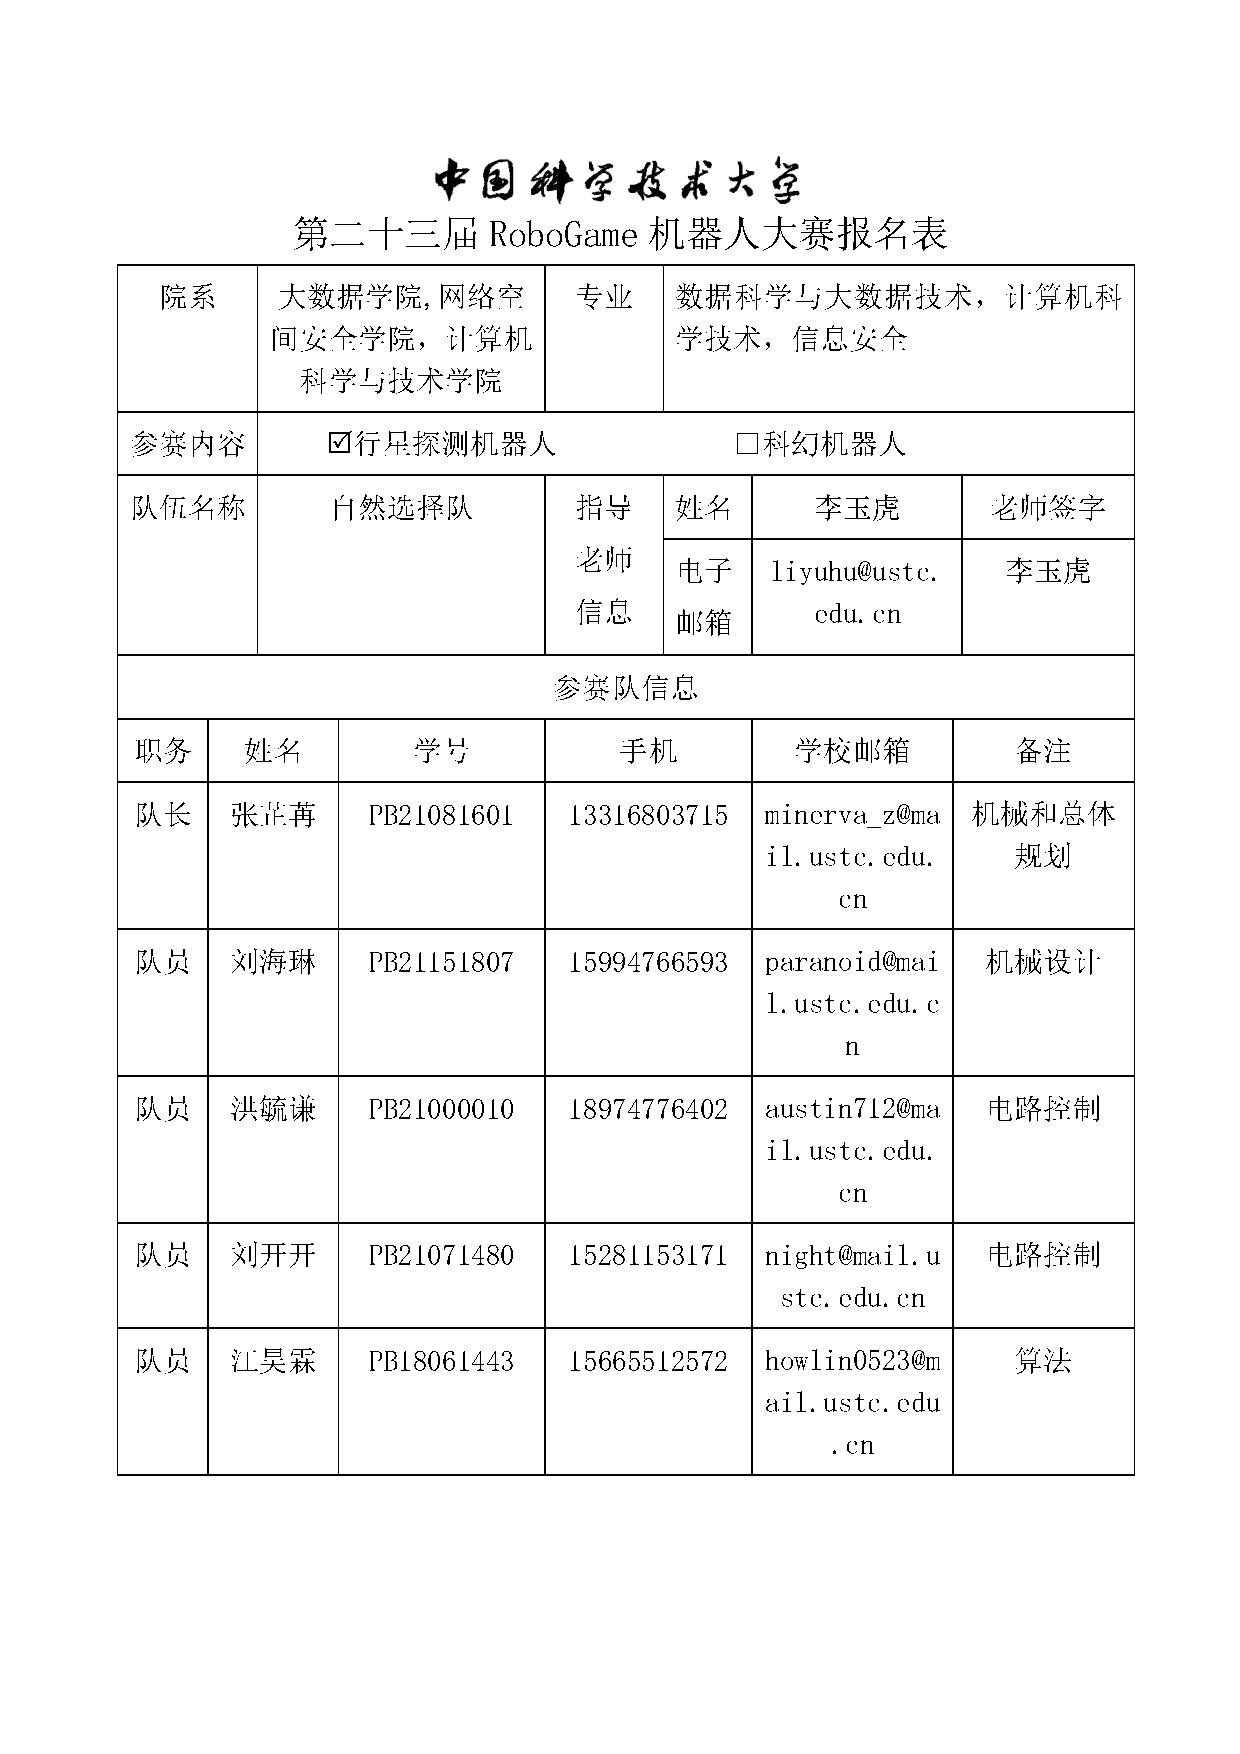
\includepdf[pages=-]{signup.pdf}

\begin{titlepage}
    \begin{center}
        \noindent
        \textcolor{black}{
\includegraphics[width=0.7\textwidth]{ustc/ustc_logo_text.pdf}}
        \vfill
        \textcolor{ustcblue}{
\includegraphics[width=0.6\textwidth]{ustc/ustc_logo_fig.pdf}}
        \vfill
        {\Huge \heiti\textbf{中国科学技术大学\enspace RoboGame\enspace 2023\\
                \vspace{0.5\baselineskip}
                自然选择队\enspace 参赛计划书
            }
        }\\
        \vspace{\baselineskip}
        % \large \textbf{小组成员(依次按照组长与姓名拼音顺序):张芷苒\ 洪毓谦\ 江昊霖\ 刘海琳\ 刘开开} \\
        % \vspace{\baselineskip}
        % \large \textbf{学科专业:数据科学与大数据技术\ 信息安全\ 计算机科学与技术} \\
        % \vspace{\baselineskip}
        % \large \textbf{指导老师:李玉虎} \\
        % \vspace{\baselineskip}
        % \large \textbf{完成时间:\today}
        {\large
            \begin{tabular}{p{2cm}l}
                \textbf{小组成员:} & \underline{\makebox[10cm]{张芷苒\ 洪毓谦\ 江昊霖\ 刘海琳\ 刘开开}}    \\
                \textbf{学科专业:} & \underline{\makebox[10cm]{数据科学与大数据技术\ 信息安全\ 计算机科学与技术}} \\
                \textbf{指导老师:} & \underline{\makebox[10cm]{李玉虎老师}}                      \\
                \textbf{完成时间:} & \underline{\makebox[10cm]{\today}}                     \\
            \end{tabular}
        }
    \end{center}
\end{titlepage}




\thispagestyle{empty}

\clearpage
\setcounter{page}{1}
\pagenumbering{roman}
\tableofcontents
\clearpage
\setcounter{page}{1}
\pagenumbering{arabic}



\section{队伍简介}
\subsection{队名介绍}

标志着这只队伍在自然选择的严苛条件下,努力实现自我突破脱颖而出。
面对严酷的竞争环境和各种挑战,这支队伍不断努力,寻找突破的机会和方法。他们付出了巨大的努力和坚定的意志,致力于提高自身的能力和竞争力。每一次挫折和困难都成为他们前进的动力,激发着他们不断探索和改进的决心。这支队伍充满着创造力和冒险精神,他们不畏艰难,不断尝试新的策略和方法,为了达到目标而不懈努力。尽管成功还没有到来,但团队的奋斗精神和毅力将为他们创造更多机会,并最终实现自我突破。

\subsection{成员(按任务分工顺序)介绍与分工}

\begin{table}[H]
    \centering
    \caption{成员介绍与分工}
    \begin{tabular}{ccc}
        \toprule
        学号         & 姓名  & 分工                                \\
        \midrule
        PB21081601 & 张芷苒 & 队长,负责全队任务安排与整体规划;机械设计,机械选型与探测车的装造 \\
        % \hline
        PB21151807 & 刘海琳 & 具体机械结构设计,机械图纸绘制                   \\
        % \hline
        PB21000010 & 洪毓谦 & 整体电路设计连接和分电设计及主控电源等模块的选型工作        \\
        % \hline
        PB21071480 & 刘开开 & 电控具体流程设计,电路控制程序设计                 \\
        % \hline
        PB18061443 & 江昊霖 & 视觉与控制算法设计及优化;计划书排版                \\
        \bottomrule
    \end{tabular}
    \label{tab:member}
\end{table}

\clearpage
\section{机械部分}
\subsection{功能与结构概述}

本次比赛要求机器人从飞船区出发,经过巡线区,斜坡区或陨石区之后到达采矿区正确识别并夹取规定数量和位置的晶体矿和燃料矿,然后返回飞船区卸下矿石,开始下一次采矿。
在可选择的三条路线(陡坡,缓坡,陨石区)中,本组经过考量决定第一二次采矿经过\SI{45}{\degree}高难度斜坡的方式到达矿山平台上,在ABD矿脉采矿;第三次经过陨石区,前往平地矿区,在矿脉CE采矿。具体而言涉及机械结构的包括以下任务:

\begin{itemize}
    \item 自动巡线
    \item 上下\SI{45}{\degree}斜坡
    \item 识别陨石并避开
    \item 识别矿物并夹取
    \item 携带矿石返回
    \item 将矿石放入正确的装载位
\end{itemize}

本组经过对比赛任务的解读和反复的商定,基本确定了机器人机械结构设计的大体布局,初步建模并修改、调整后,得到基本模型如下:
\begin{figure}[H]
    \centering
    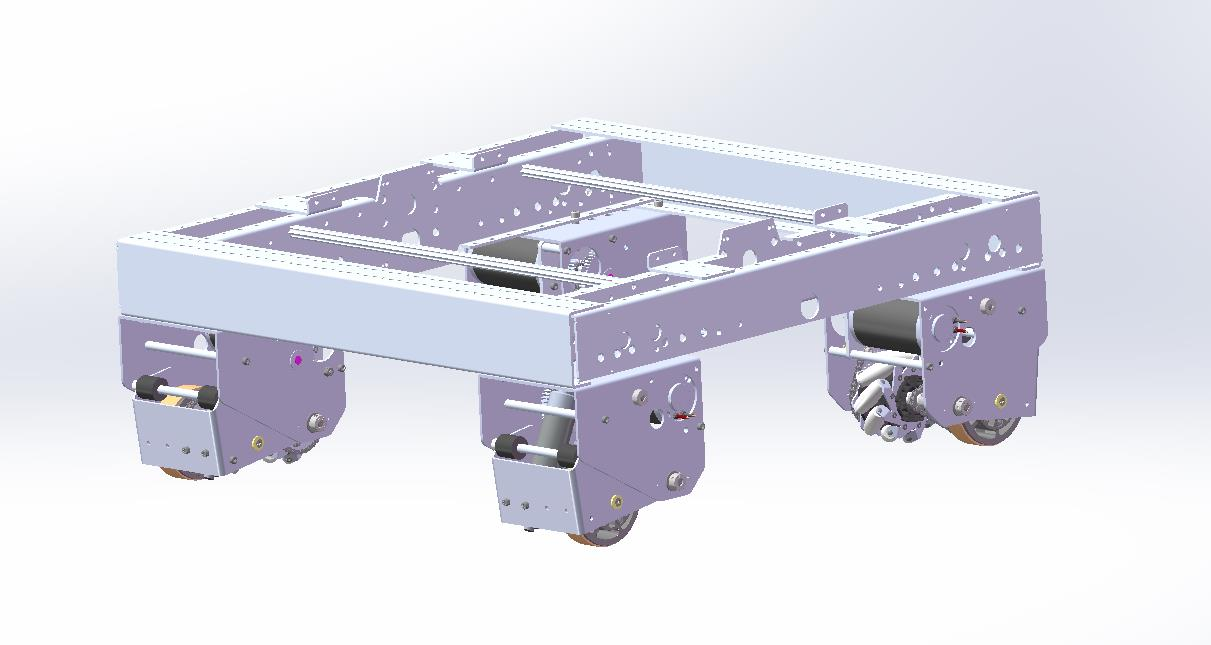
\includegraphics[width = 0.8\textwidth]{machinery/carbody.jpg}
    \caption{车体斜俯视图}
    \label{fig:carbody}
\end{figure}



\subsection{模块设计与选型}
\subsubsection{底盘}
\begin{enumerate}
    \item 架构:由于本次比赛无越障任务且除了上下坡之外地面平坦,所以选择无悬挂以降低设计复杂度。同时,考虑到车身长度至少为\SI{300}{\milli\meter},而\SI{45}{\degree}斜坡的底宽只有\SI{200}{\milli\meter},为避免在上下坡时车身长度大于斜坡坡面长度导致坡与平地连接处触及底盘,我们采取了架高底盘的策略,将底盘完全架于轮子之上。
          \begin{figure}[H]
              \centering
              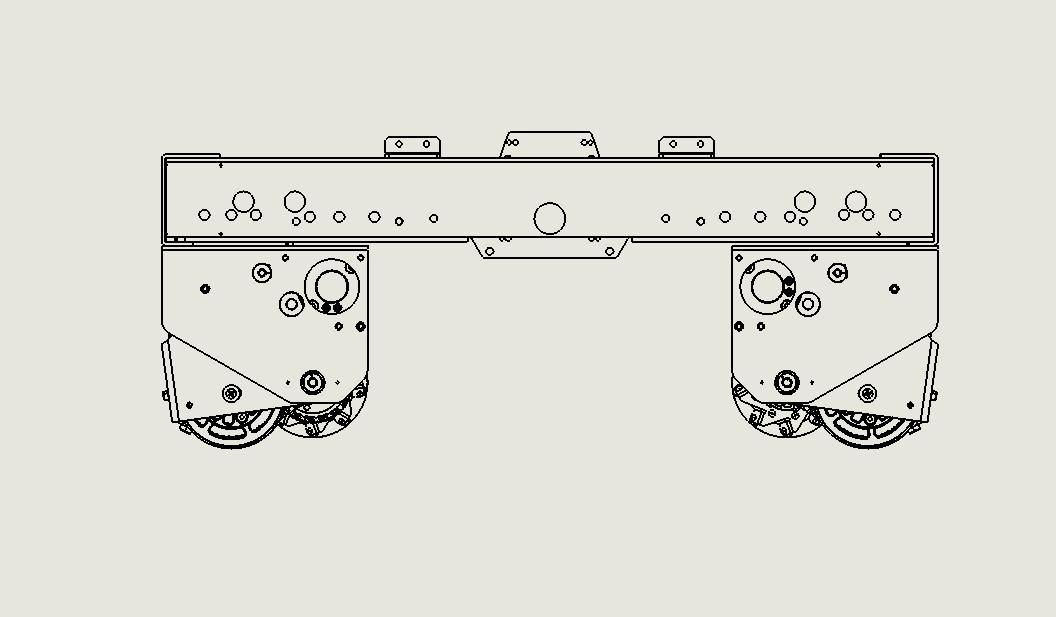
\includegraphics[width = 0.7\textwidth]{machinery/car_left.jpg}
              \caption{车体左视图}
              \label{fig:car_left}
          \end{figure}
          \begin{figure}[H]
              \centering
              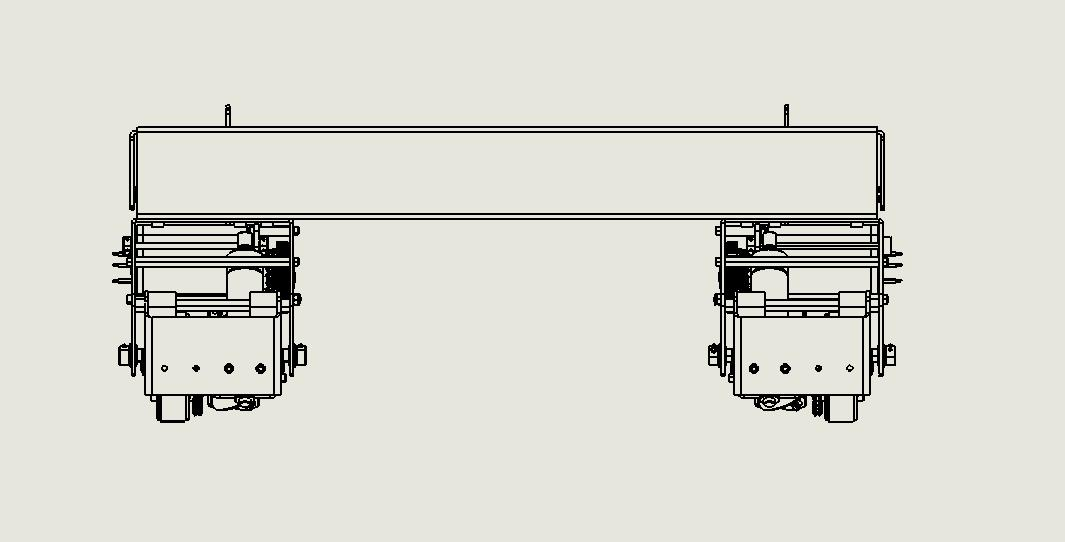
\includegraphics[width = 0.7\textwidth]{machinery/car_front.jpg}
              \caption{车体正视图}
              \label{fig:car_front}
          \end{figure}
    \item 底盘:取放矿石及运回过程需要用到机械抓取臂以及一能装载三个矿石的容器,因此底盘需要有较大的强度并且尽量轻,以降低车身自重。由于对爬坡要求高,希望车的重心落于偏后方。基于这两点,我们采用$300\si{\milli\meter} \times 350\si{\milli\meter}$的铝框作为主体。铝合金材料较为轻量化但强度高,可以保证结构的稳定性和刚性。在承重部分,我们在需要安置机械臂和电池组模块的位置再铺上\SI{5}{\milli\meter}厚碳板作为支撑,底部用两根铝条进行支撑。
          \begin{figure}[H]
              \centering
              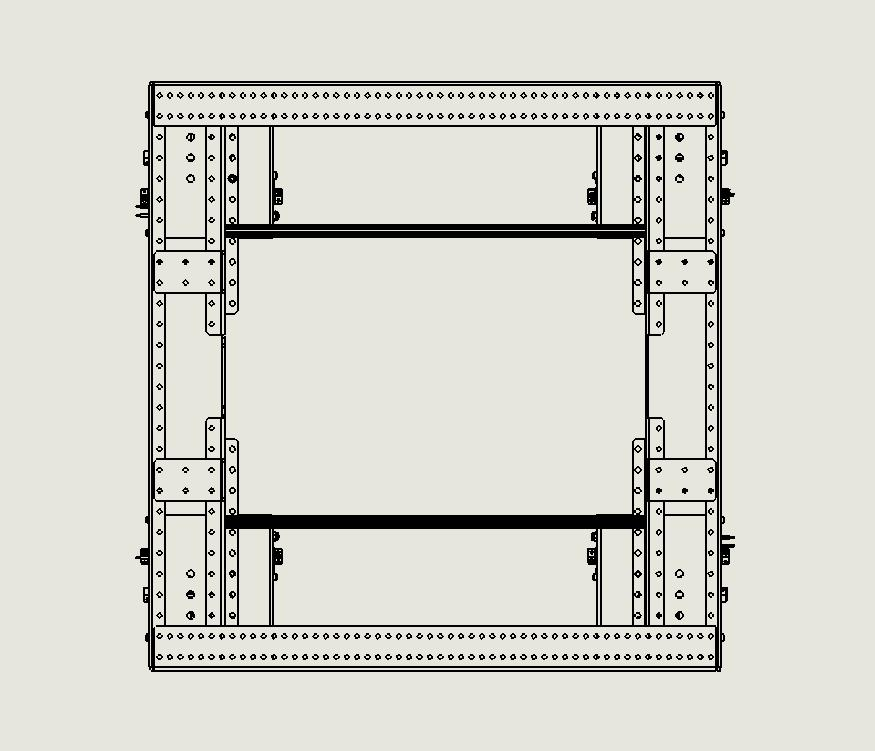
\includegraphics[width = 0.55\textwidth]{machinery/car_top.jpg}
              \caption{车体俯视图}
              \label{fig:car_top}
          \end{figure}
\end{enumerate}

\subsubsection{轮组}
\subsubsubsection{主驱动}
\par
为了确保爬坡抓地力,同时兼顾在不同矿脉之间的转向以及保证巡线时的方向变动足够灵活,
本组决定采用四组中心对称、每组一个胶轮与一个麦轮相连接的轮组作为主驱动。麦轮由一组斜向排列的轮胎组成,使得轮胎的旋转方向能够相互垂直,从而实现任意方向上的平移,增加灵活性。而胶轮可以增加车子在爬坡时候的摩擦力,避免翻倒或者打滑。效果图如下:
\begin{figure}[H]
    \centering
    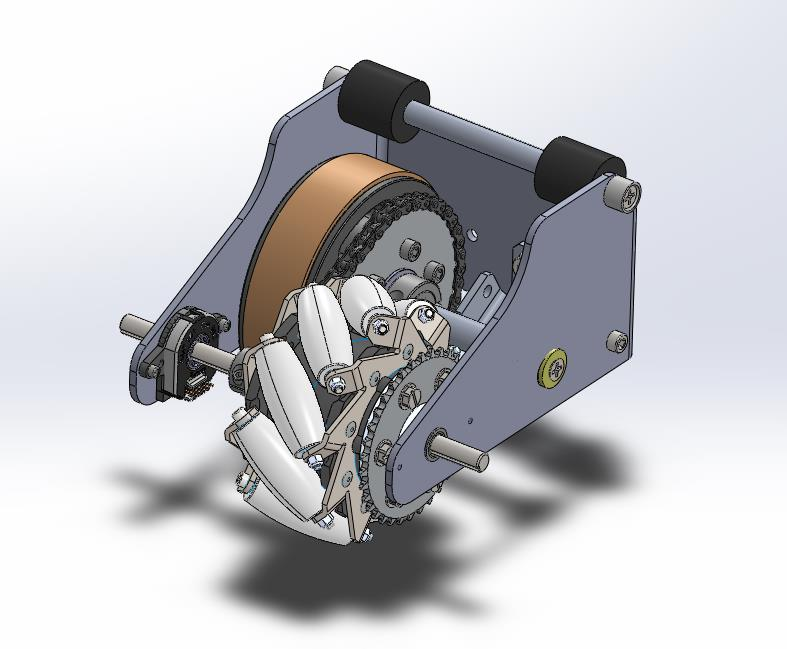
\includegraphics[width = 0.6\textwidth]{machinery/wheel.jpg}
    \caption{轮子斜俯视图}
    \label{fig:wheel}
\end{figure}
\par
520编码直流电机对四个麦轮进行直接驱动,麦轮再通过齿轮与胶轮进行联动。
我们还在轮组的周围设置了保护罩来防止意外接触造成的伤害。
为了保持车的重心较低,考虑到我们的底盘比较高,我们选用尺寸较小的\SI{100}{\milli\meter}直径麦轮与胶轮。
\par
单个轮组由1个麦克纳姆轮(100mm直径)、1个橡胶轮(100mm直径)、1个AMT103编码器、3个齿轮(参数分别为模数0.85英尺齿数14、模数0.025英尺齿数50、模数0.025英尺齿数14)、3个铝合金板、若干螺母(M10-32)、若干螺钉等零部件组成。单个轮组俯视图如下所示:
\begin{figure}[H]
    \centering
    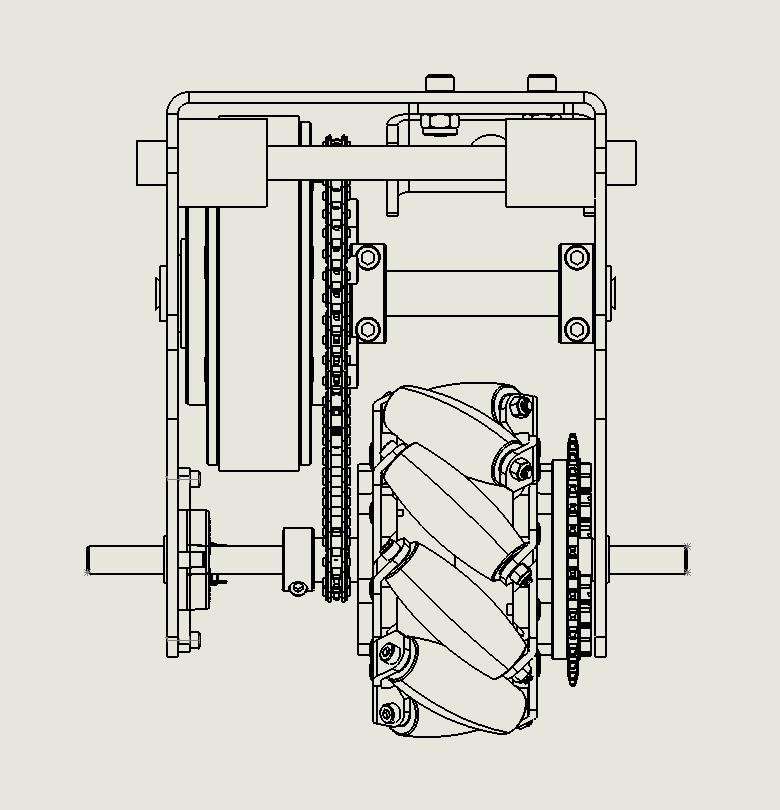
\includegraphics[width = 0.6\textwidth]{machinery/wheel_top.jpg}
    \caption{轮子俯视图}
    \label{fig:wheel_top}
\end{figure}
\subsubsubsection{辅助}
\par
本组选择了爬\SI{45}{\degree}坡抵达矿脉的路线。在研究了不同的爬坡方案后,我们决定采取以下措施来完成任务:增加动力输出、降低并向后移动重心,并在车辆尾部延长加装支撑轮,以避免牛顿第三定律导致车辆后翻的风险。
为了保证车在上坡时不会发生后翻的现象,考虑在车尾安装直径小于主驱动轮的无动力辅助支撑胶轮。
由于截至计划书提交尚未进行过实验,所以此部分没有画进最终的设计中。计划在初步组装车体,进行上坡实验之后,再考虑此部分的添加。
若此方案不能满足要求,将会考虑在上坡时使用喷气推进系统作为动力辅助。
\subsubsection{抓取结构}
\par
取放矿石需要机械臂和机械爪来进行。
为了保证在行进过程中车辆重心不会太高,在抵达矿脉或装载区之前机械臂保持折叠状态,需要取矿或放矿时再展开。
为了方便停在一个位置时就可以从不同的矿坑里抓取矿石,
以及抓取矿石后投入车身装载装置,机械臂的底盘需要可以旋转。
\par
机械臂由1个合金大底板、1个合金金属旋转底座、2个铝合金U支架、1个深沟球轴承、1个LD-1501MG舵机(用于底座)、2个LDX-218舵机(用于手臂)、2个LFD-06舵机(用于手臂)、1个LDX-335MG舵机(用于机械爪)、1个主金属舵盘、1个主塑料舵盘、1个副塑料舵盘、1个三合一开发板、若干螺钉螺母等零部件组成。
下图为机械臂设计图:
\begin{figure}[H]
    \centering
    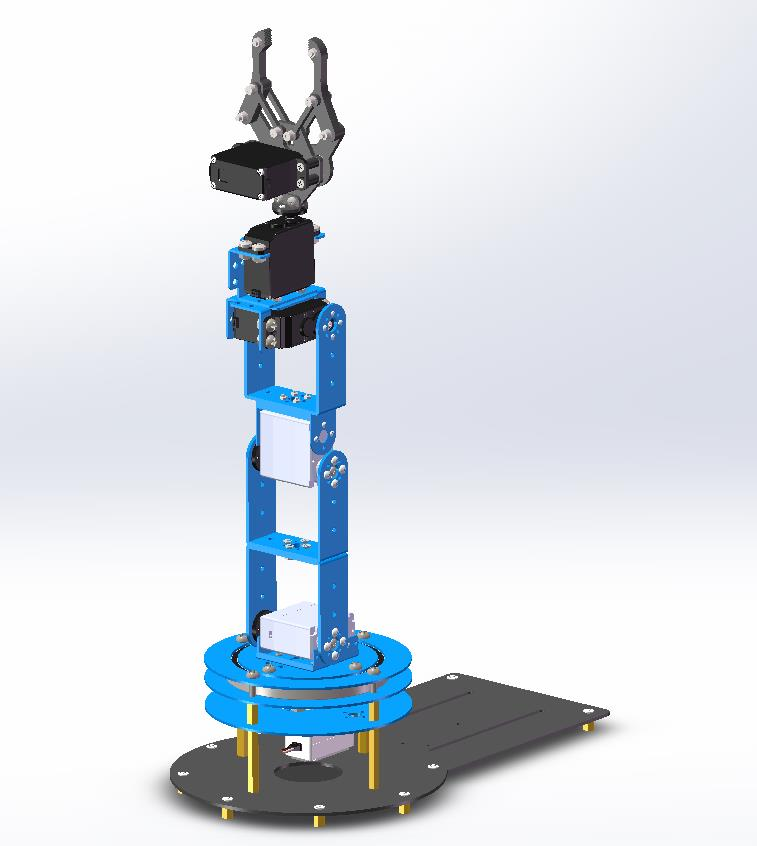
\includegraphics[width = 0.9\textwidth]{machinery/arm.jpg}
    \caption{机械臂斜俯视图}
    \label{fig:arm}
\end{figure}
%%拼图
\vfill
\begin{figure}[H]
    \centering
    \begin{subfigure}{0.45\textwidth}
        \centering
        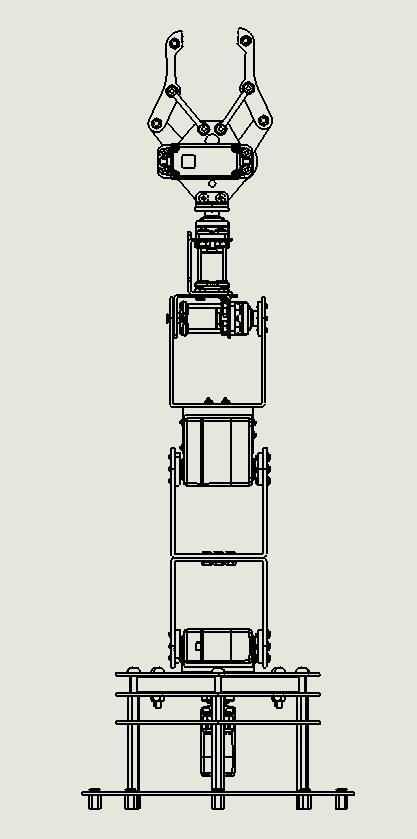
\includegraphics[width = 0.6\textwidth]{machinery/arm_front.jpg}
        \caption{正视图}
    \end{subfigure}
    \begin{subfigure}{0.45\textwidth}
        \centering
        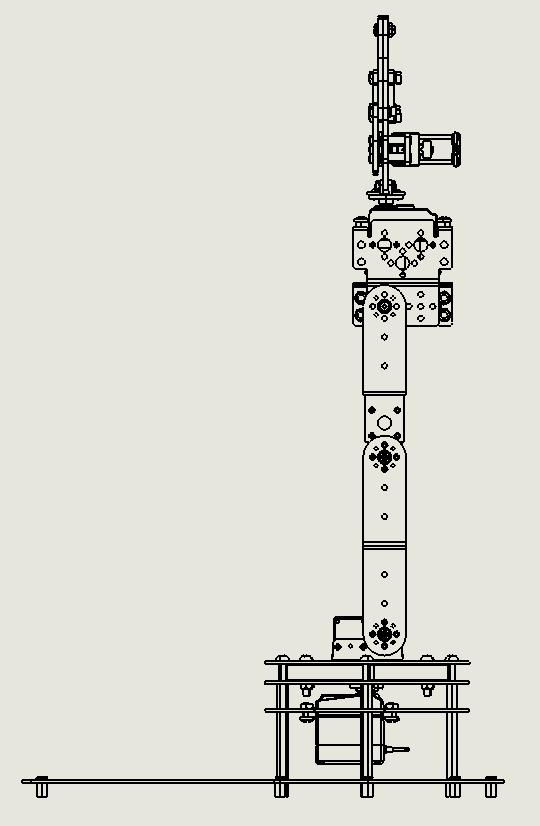
\includegraphics[width = 0.6\textwidth]{machinery/arm_left.jpg}
        \caption{侧视图}
    \end{subfigure}
    \caption{机械臂正视图和侧视图}
\end{figure}

\par
该机械臂由底座、中部、顶部、机械爪四处舵机控制。底座使用 Deep groove ball bearing(深沟球轴承)来保证转向灵活度,其他部位主材质为铝材或钢材。底部舵机使用了LD-1501MG大扭矩舵机,可以支持\SI{180}{\degree}旋转。
中部舵机架在两级支架上,控制机械臂的张合。顶部舵机控制机械爪的深探角度。机械爪舵机来控制其开合与夹取,各部分之间由螺丝连接,结构较为简单。机械爪使用的LDX-335MG舵机具有防堵转功能,当发生堵转的时候,舵机会自动计时。当堵转超过4分钟时,舵机会自动停止工作。
\par
在参考其他设计后,本组的机械爪开合由被舵机驱动的左右两个对称的带齿轮摇杆控制,带动上面两杆进行抓取。

\begin{figure}[H]
    \centering
    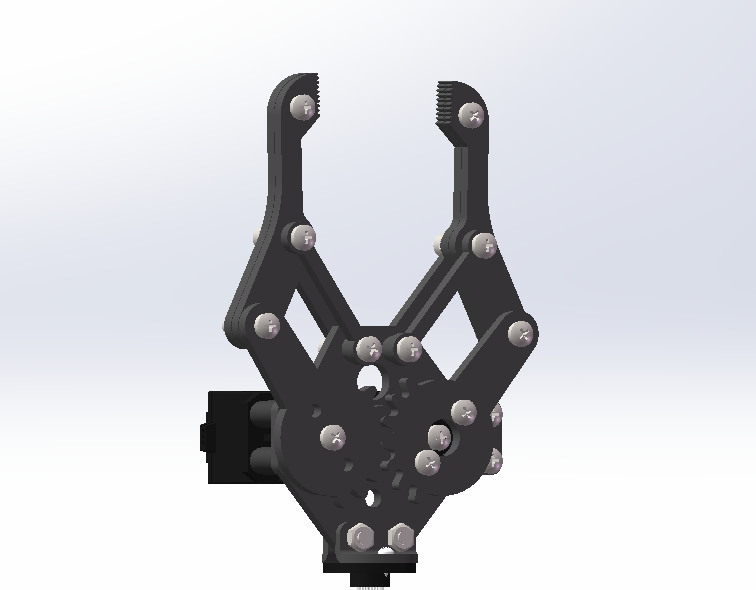
\includegraphics[width = 0.5\textwidth]{machinery/claw.png}
    \caption{机械爪}
    \label{fig:claw}
\end{figure}
\clearpage
\subsubsection{其他结构}
\par
机器人需要上下陡坡,因此希望其重心落于车辆中偏后部,故计划将电池组,电机,芯片等固件安放于底盘上偏后位置,以平衡前部机械臂,放置矿石的篮子等的重量。后续将根据机械臂结构实际重量合理安排机器人的质量分配,可能需要加装配重块 。

\clearpage
\section{电路部分}
\subsection{电路框图}
\begin{figure}[H]
    \centering
    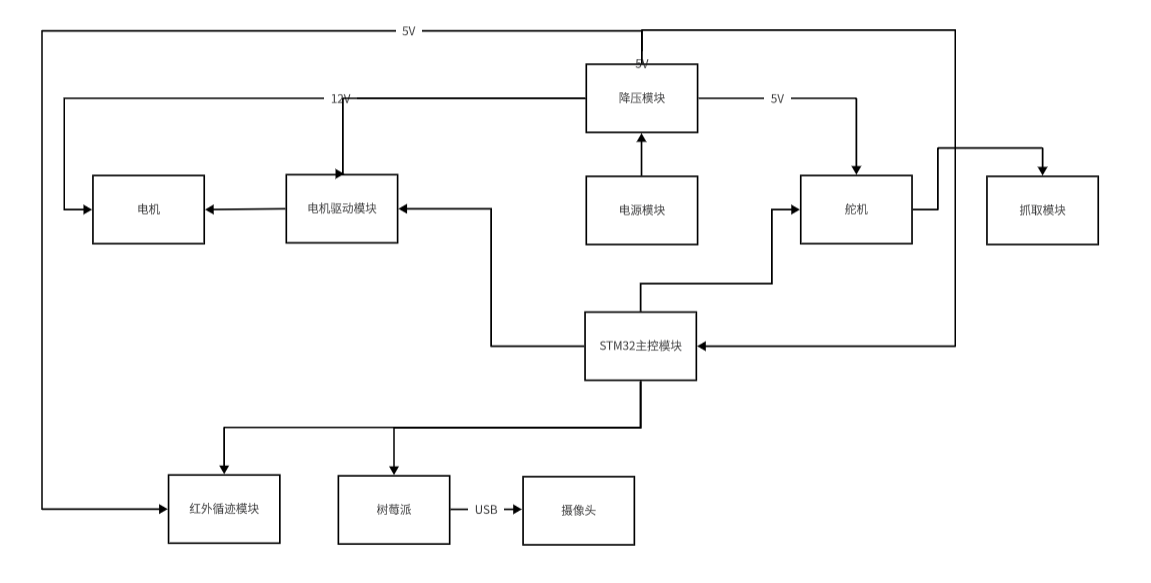
\includegraphics[width = 0.8\textwidth]{circuit.png}
    \caption{电路框图}
    \label{fig:circuit}
\end{figure}
\subsection{供电系统}
\subsubsection{电源}
电源选取\SI{24}{\volt}锂电池作为电源,工作电压范围为\SIrange{18}{25.2}{\volt}。为确保电机电压供应稳定,决定对四个驱动电机单独供电,而其他设备则共用一个主电源。

单独供电电源重量约 \SI{300}{\gram},额定容量 \SI{2600}{\milli\ampere\hour},尺寸为 $115\si{\milli\meter}\times 19\si{\milli\meter}\times 68\si{\milli\meter}$,最大持续电流不超过\SI{5}{\ampere},最大瞬间电流不超过\SI{10}{\ampere},最大支持功率不超过\SI{120}{\watt}。

\begin{figure}[H]
    \centering
    \begin{subfigure}[0]{0.44\textwidth}
        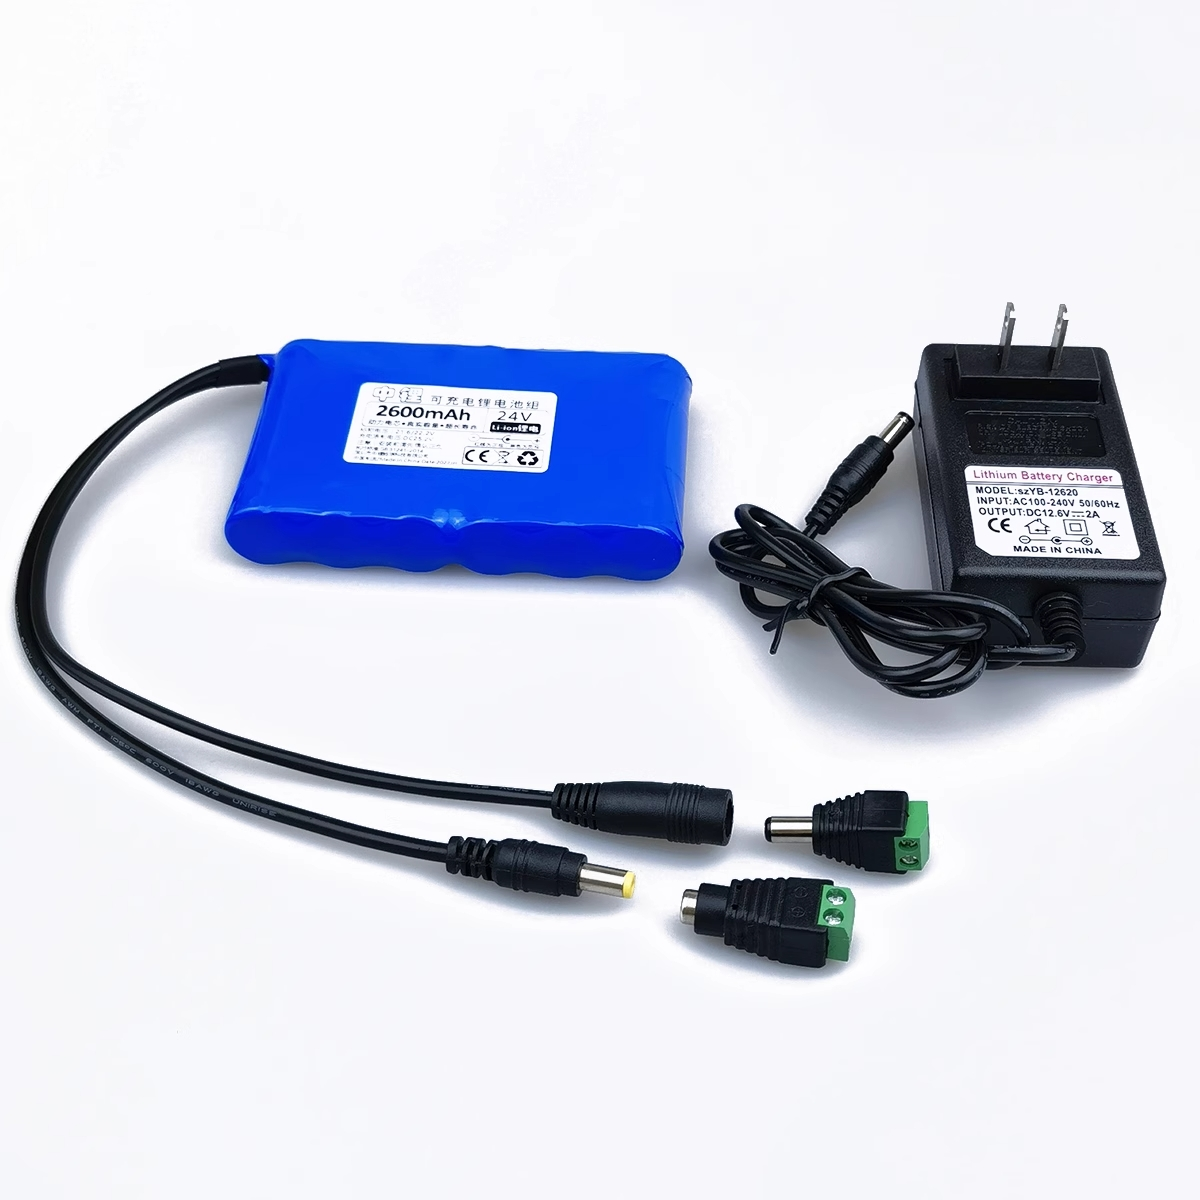
\includegraphics[width = \textwidth]{source/separate_source.jpg}
        \caption{单独供电电源}
        \label{fig:separate_source}
    \end{subfigure}
    \hfil
    \begin{subfigure}[0]{0.44\textwidth}
        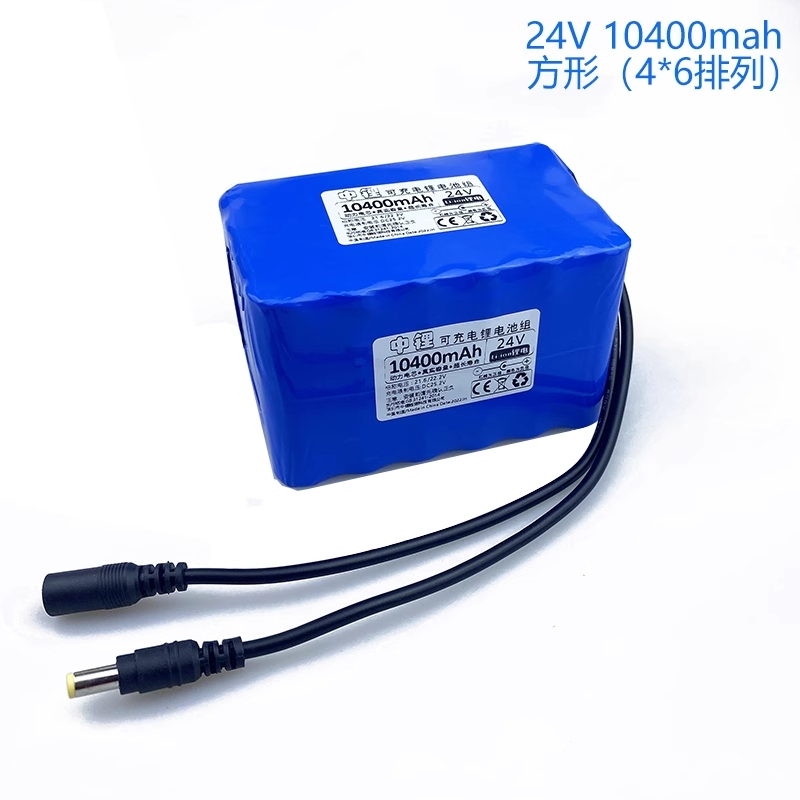
\includegraphics[width = \textwidth]{source/main_source.jpg}
        \caption{主电源}
        \label{fig:main_source}
    \end{subfigure}
    \caption{电源}
\end{figure}

% \begin{figure}[H]
%     \centering
%     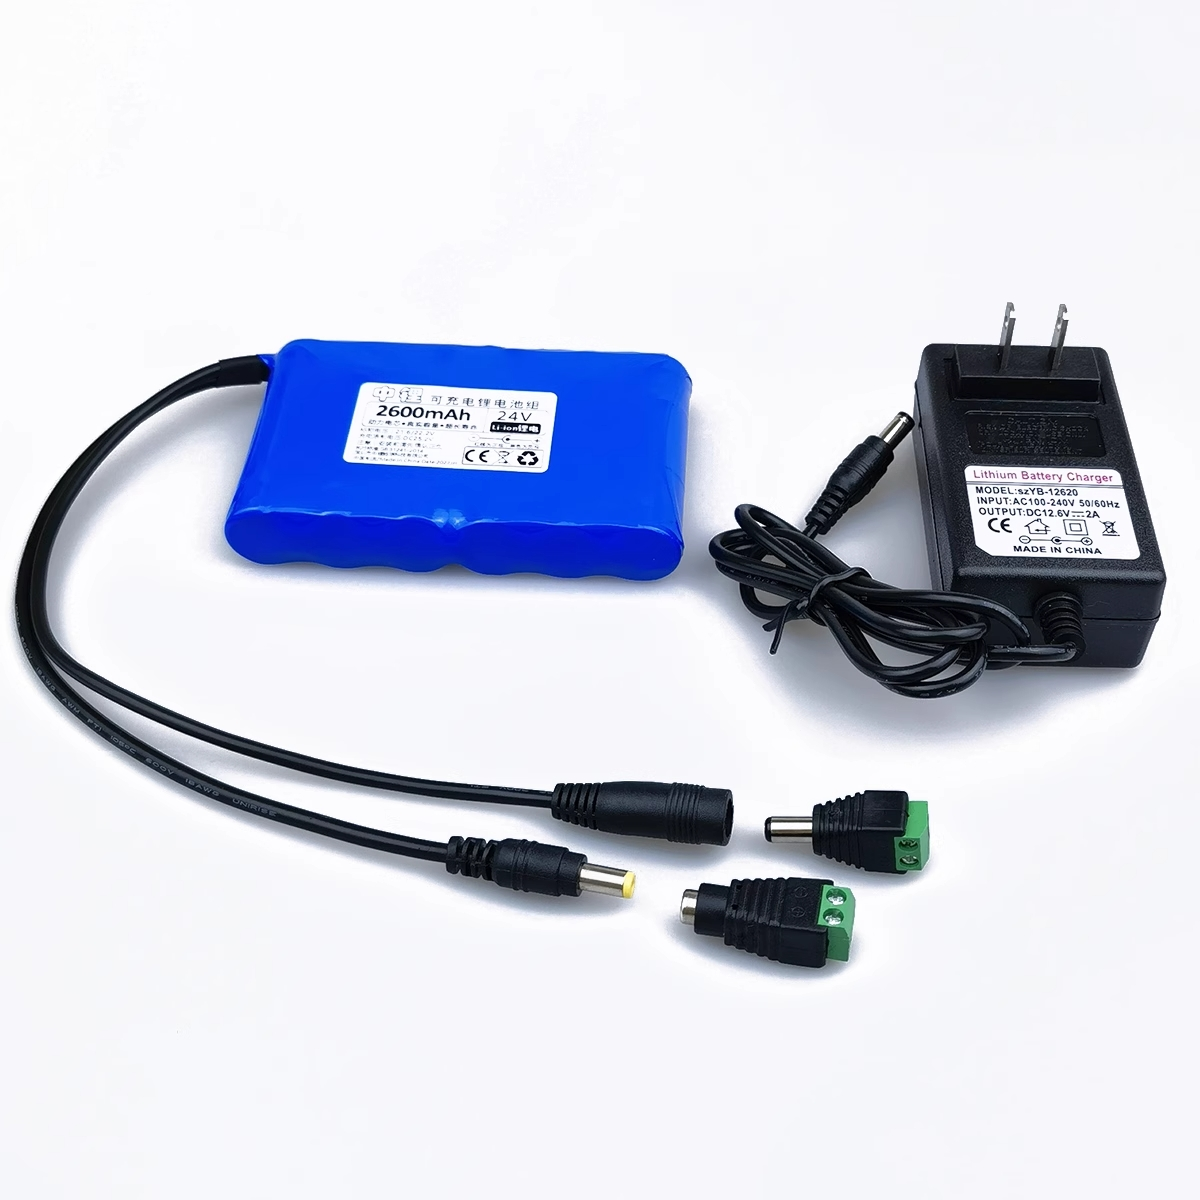
\includegraphics[width = 0.5\textwidth]{source/separate_source.jpg}
%     \caption{单独供电电源}
%     \label{fig:separate_source}
% \end{figure}

主电源的重量约为\SI{1200}{\gram},额定容量为\SI{10400}{\milli\ampere\hour},尺寸为$11576\si{\milli\meter}\times 68\si{\milli\meter}$,最大持续电流不超过\SI{10}{\ampere},最大瞬间电流不超过\SI{20}{\ampere},最大支持功率不超过\SI{240}{\watt}。
% 插入主电源图片
% \begin{figure}[H]
%     \centering
%     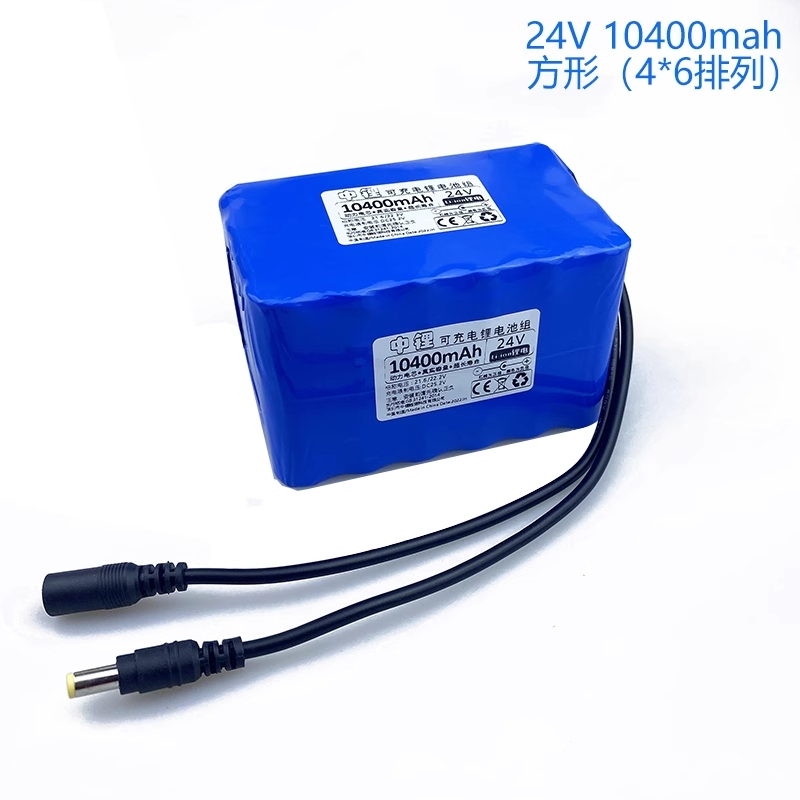
\includegraphics[width = 0.5\textwidth]{source/main_source.jpg}
%     \caption{主电源}
%     \label{fig:main_source}
% \end{figure}

\SI{24}{\volt} 电源参数图如下:

% 插入电源参数图片
\begin{figure}[H]
    \centering
    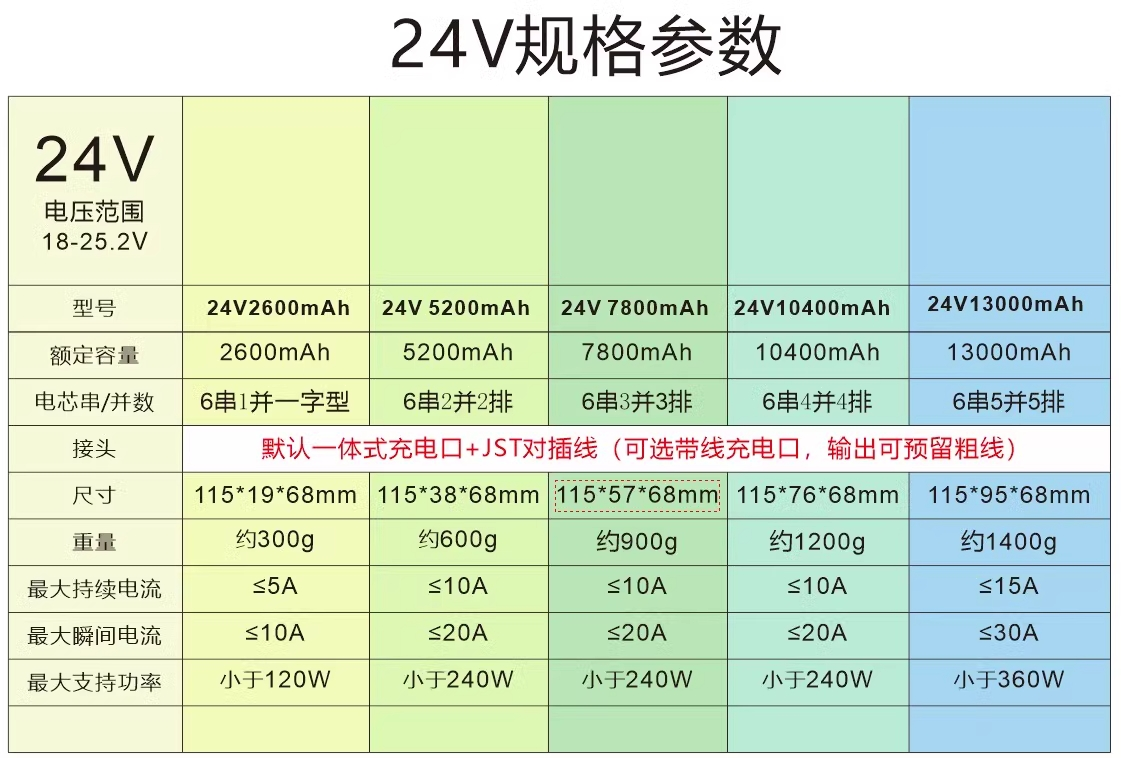
\includegraphics[width = 0.8\textwidth]{source/source_parameter.jpg}
    \caption{电源参数}
    \label{fig:source_parameter}
\end{figure}


为了保障树莓派的供电,选取目前市面上常见的充电宝作为其电源,以防出现通信问题。
\subsubsection{分电方案}
分电方案采用 Robogame 官方指定分电板。
\subsubsection{稳压方案}
由于电源电压为 \SI{24}{\volt},而电路中含有输入电压为
\SI{14.8}{\volt}、\SI{6.8}{\volt}、\SI{5}{\volt}、\SI{3.3}{\volt} 的模块和芯片,故需要使用降压模块来将较高电压转化为合适的电压。由于所需功率较大,且为了方便观察输出电压,所以我们选择以下这款 DC-DC 电源管理模块实现上述功能。

% 插入稳压模块图片
\begin{figure}[H]
    \centering
    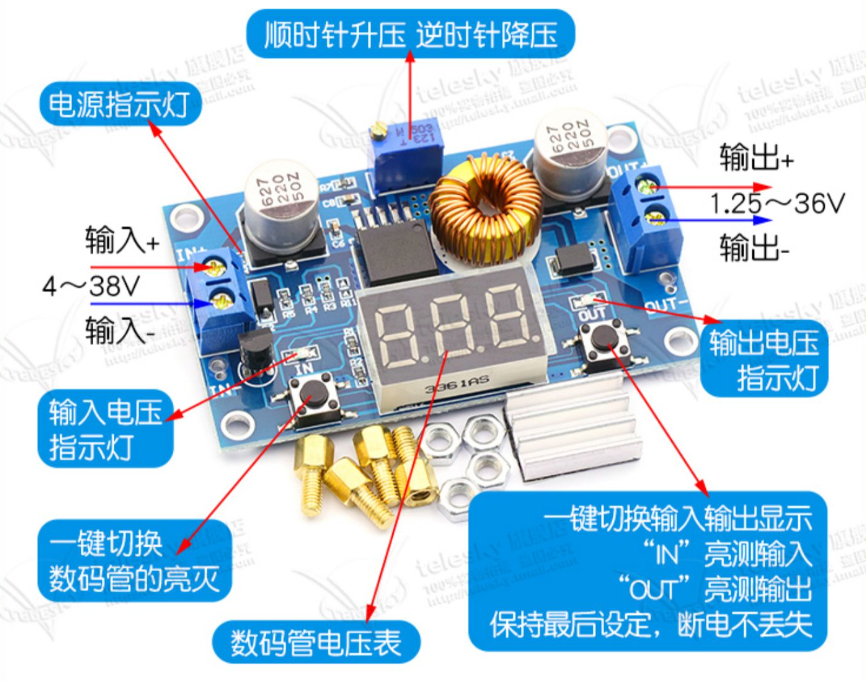
\includegraphics[width = 0.5\textwidth]{stabilivolt/stabilivolt.png}
    \caption{稳压模块}
    \label{fig:stabilivolt}
\end{figure}

产品特点:

\begin{figure}[H]
    \centering
    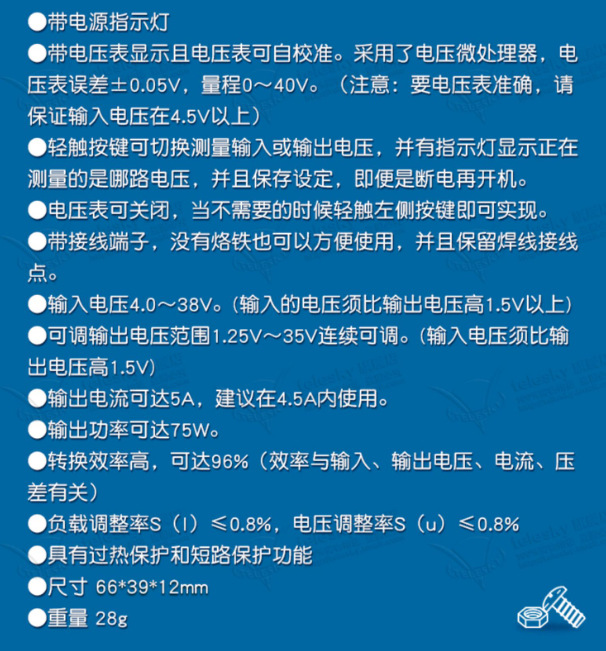
\includegraphics[width = 0.5\textwidth]{stabilivolt/stabilivolt_parameter.png}
    \caption{稳压模块参数}
    \label{fig:stabilivolt_parameter}
\end{figure}


\subsection{控制系统}
\subsubsection{主控模块}
\textbf{STM32F407简介}:STM32F407系列MCU面向需要在小至$10\si{\milli\meter}\times 10 \si{\milli\meter}$的封装内实现高集成度、高性能、嵌入式存储器和外设的医疗、工业与消费类应用。STM32F407 MCU提供了工作频率为168 MHz的Cortex™-M4内核(具有浮点单元)的性能。



\begin{itemize}
    \item 性能:在168 MHz频率下,从Flash存储器执行时,STM32F407单片机能够提供210 DMIPS/566 CoreMark性能,并且利用意法半导体的ART加速器实现了FLASH零等待状态。DSP指令和浮点单元扩大了产品的应用范围。
    \item 功效:该系列产品采用意法半导体\SI{90}{\nano\meter}工艺和ART加速器,具有动态功耗调整功能,能够在运行模式下和从Flash存储器执行时实现低至$238\mu\si{ \ampere/\mega\hertz}$的电流消耗。
    \item 丰富的连接功能:与STM32F4x5系列相比,STM32F407单片机还具有符合IEEE 1588 v2标准要求的以太网MAC10/100和能够连接CMOS照相机传感器的8~14位并行照相机接口。
    \item 2个USB OTG(其中一个支持HS)
    \item  音频:专用音频PLL和2个全双工I²S
    \item  通信接口多达15个(包括6个速度高达11.25 Mb/s的USART、3个速度高达45 Mb/s的SPI、3个I²C、2个CAN和1个SDIO)
    \item  模拟:2个12位DAC、3个速度为2.4 MSPS或7.2 MSPS(交错模式)的12位ADC
    \item  定时器多达17个:频率高达168 MHz的16和32位定时器
    \item  可以利用支持Compact Flash、SRAM、PSRAM、NOR和NAND存储器的灵活静态存储器控制器轻松扩展存储容量
    \item  基于模拟电子技术的真随机数发生器
    \item STM32F407产品系列具有\SI{512}{K\byte}~\SI{1}{M\byte}的Flash和\SI{192}{K\byte}的SRAM,采用尺寸小至$10\si{\milli\meter} \times 10 \si{\milli\meter}$的\SIrange{100}{176}{}引脚封装。
\end{itemize}






综合考虑,主控模块采用正点原子STM32F407ZGT6系统板,此系统板足以胜任比赛要求。

\begin{figure}[H]
    \centering
    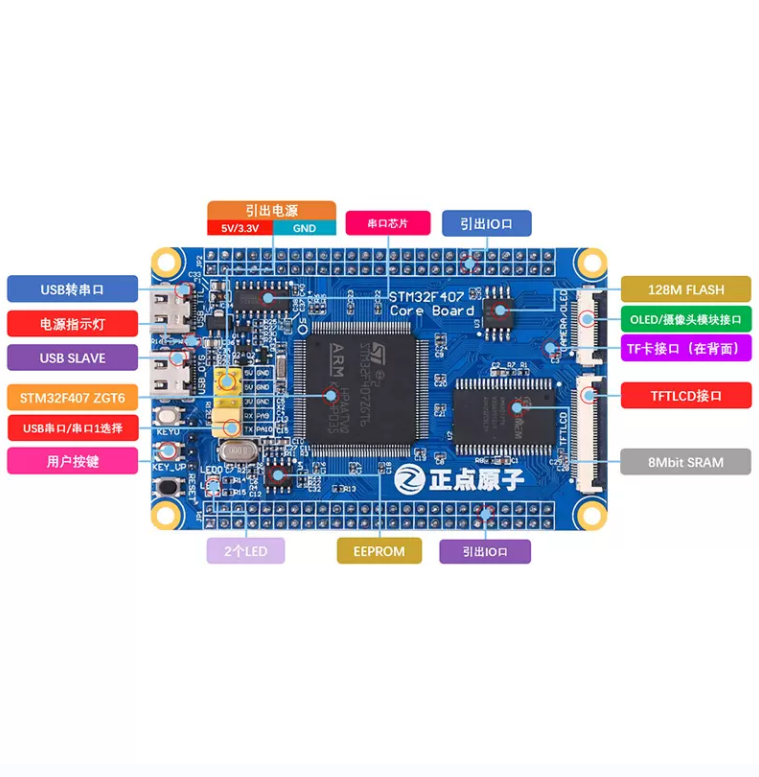
\includegraphics[width=0.6\textwidth]{control/control.png}
    \caption{主控模块}
    \label{fig:control}
\end{figure}

STM32F407ZGT6系统板结构尺寸图如下:

\begin{figure}[H]
    \centering
    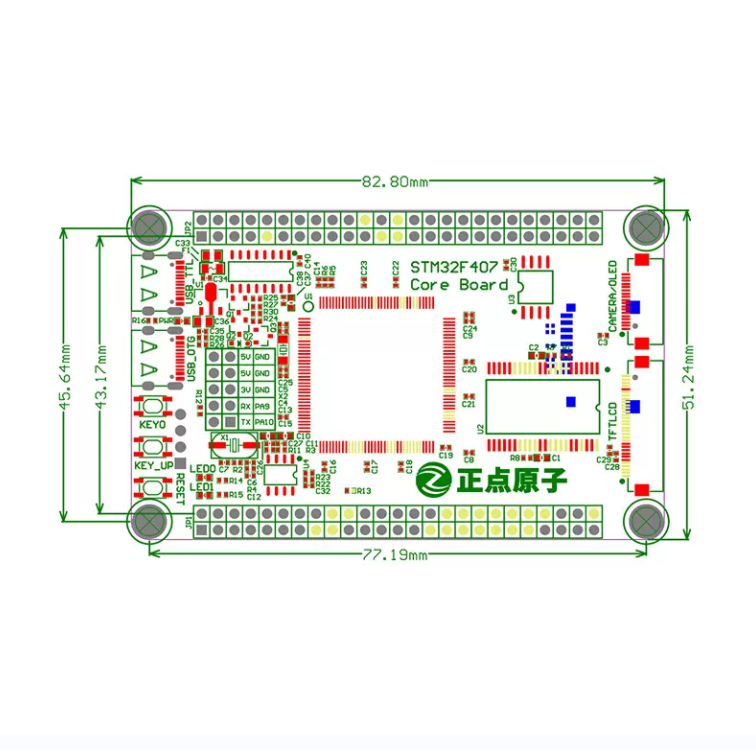
\includegraphics[width=0.6\textwidth]{control/control_parameter1.png}
    \caption{主控模块结构尺寸图}
    \label{fig:control_parameter1}
\end{figure}

STM32F407ZGT6系统板各项参数如下:

\begin{figure}[H]
    \centering
    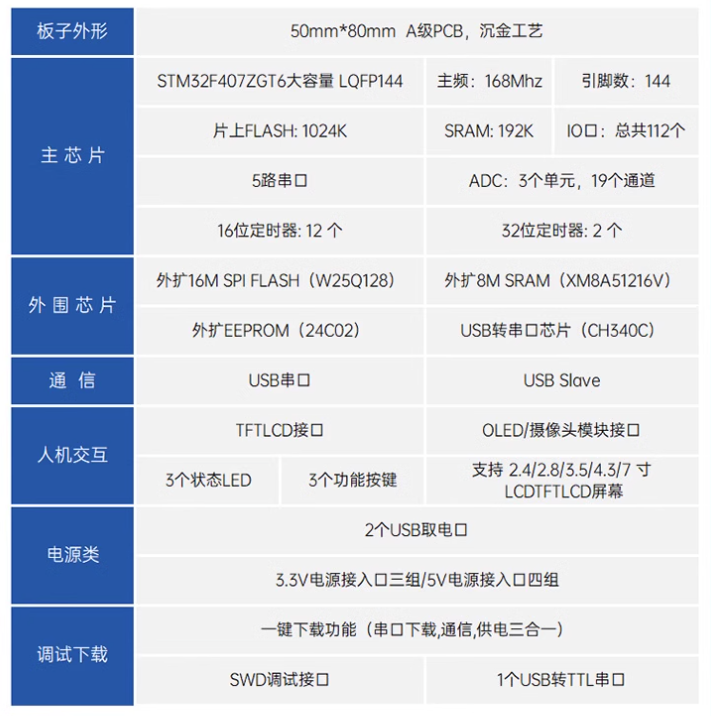
\includegraphics[width=0.6\textwidth]{control/control_parameter2.png}
    \caption{主控模块参数图}
    \label{fig:control_parameter2}
\end{figure}

% 主控模块参数图2
\subsubsection{计算平台}
树莓派(英文:Raspberry Pi)是基于 Linux 的单片机电脑,还有一般电脑没有的接口,GPIO 接口,这是一套通用的 IO 接口,树莓派通过这些 GPIO 引脚可以跟很多传感器进行通信,也就是读取和控制。还可以安装 ARM 架构的操作系统。

相比上一代的树莓派3B+,树莓派4B在处理器速度,多媒体性能,内存和连接方面提供了突破性的增长,同时保留了后向兼容性和类似的功耗。对用户来说,树莓派4B提供的桌面性能可与入门级x86 PC系统相媲美。树莓派4B的主要功能包括高性能64位四核处理器,通过一对micro-HDMI端口支持分辨率高达4K的双显示屏,高达4Kp60的硬件视频解码,4GB的RAM,双频2.4/5.0 GHz无线局域网,蓝牙5.0,千兆以太网,USB 3.0和PoE功能(通过单独的PoE HAT插件)。双频无线局域网和蓝牙具有模块化合规认证,允许将电路板设计到最终产品中,大大降低了合规性测试,从而降低了成本和上市时间。

综合考虑,选取树莓派4B作为计算平台。

\begin{figure}[H]
    \centering
    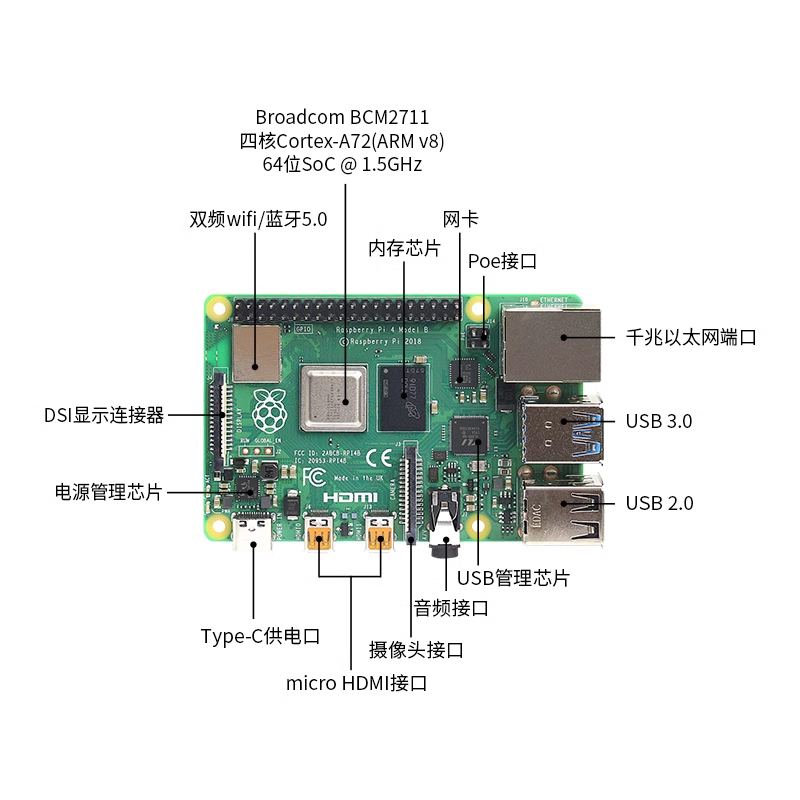
\includegraphics[width=0.6\textwidth]{raspberrypi/raspberry_pi.png}
    \caption{计算平台}
    \label{fig:raspberry_pi}
\end{figure}

树莓派4B和树莓派3B+参数图如下:

\begin{figure}[H]
    \centering
    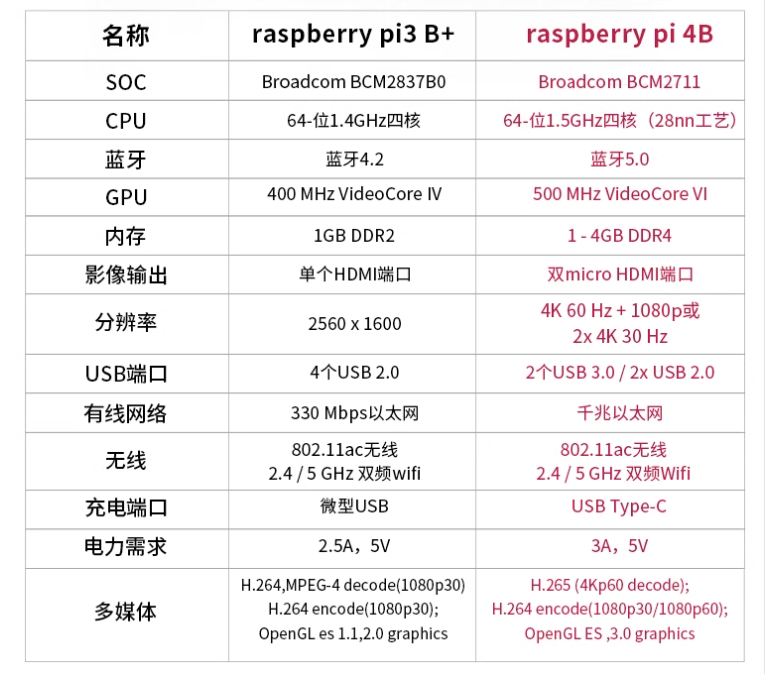
\includegraphics[width=0.6\textwidth]{raspberrypi/raspberry_pi_parameter.png}
    \caption{树莓派4B和树莓派3B+参数图}
    \label{fig:raspberry_pi_parameter}
\end{figure}
\subsection{执行系统}

\subsubsection{电机}


选择直流有刷电机520编码器电机,电压 \SI{12}{\volt},减速比 1:30,额定转矩 \SI{3.5}{\kilogram\cdot\centi\meter},额定电流 \SI{1}{\ampere},额定转速 \SI{250}{\rpm}。



\begin{figure}[H]
    \centering
    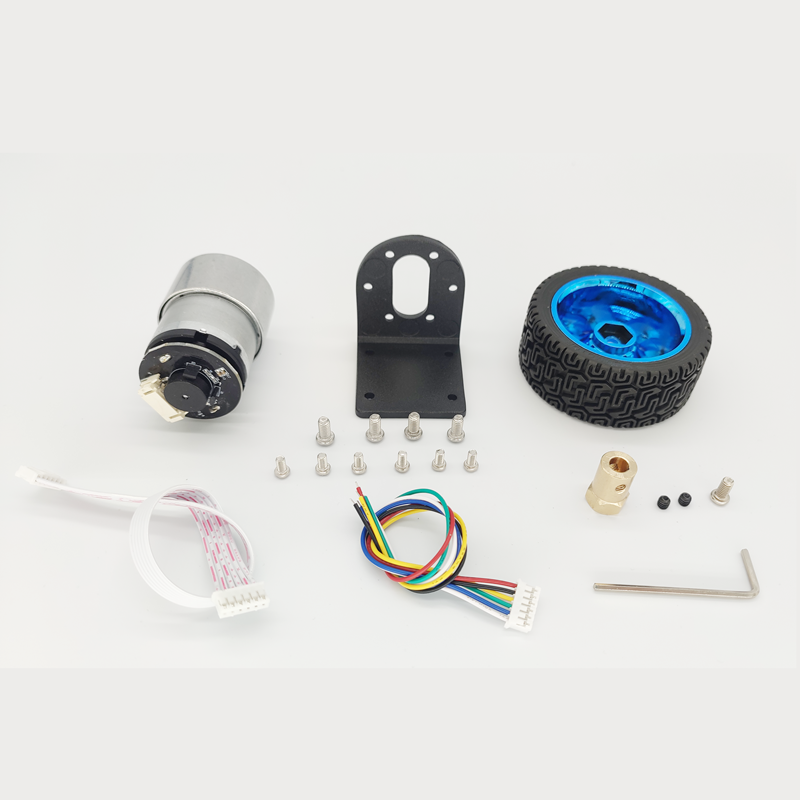
\includegraphics[width=0.6\textwidth]{motor/motor.png}
    \caption{电机实物图}
    \label{fig:motor}
\end{figure}

\begin{figure}[H]
    \centering
    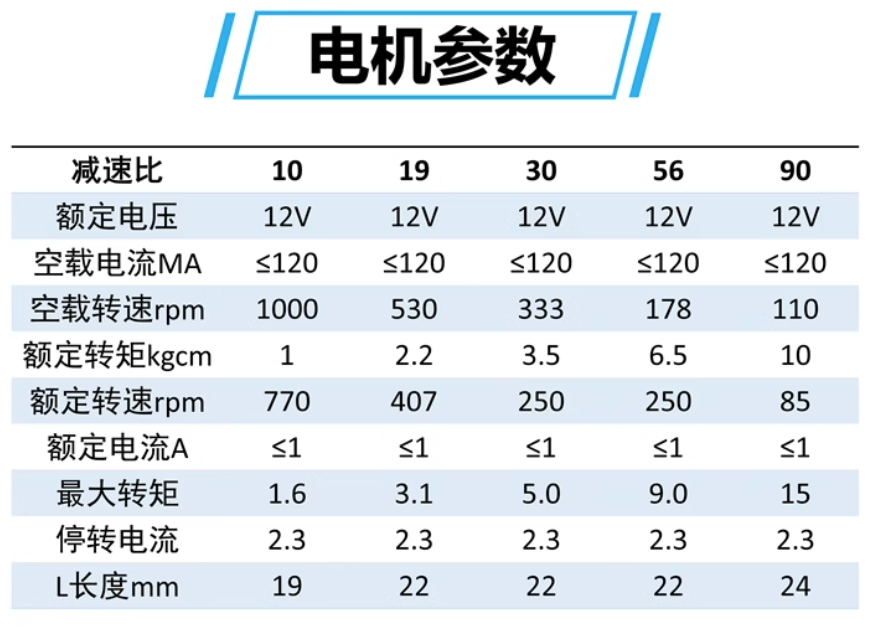
\includegraphics[width=0.6\textwidth]{motor/motor_parameter1.png}
    \caption{电机参数图}
    \label{fig:motor_parameter1}
\end{figure}

\begin{figure}[H]
    \centering
    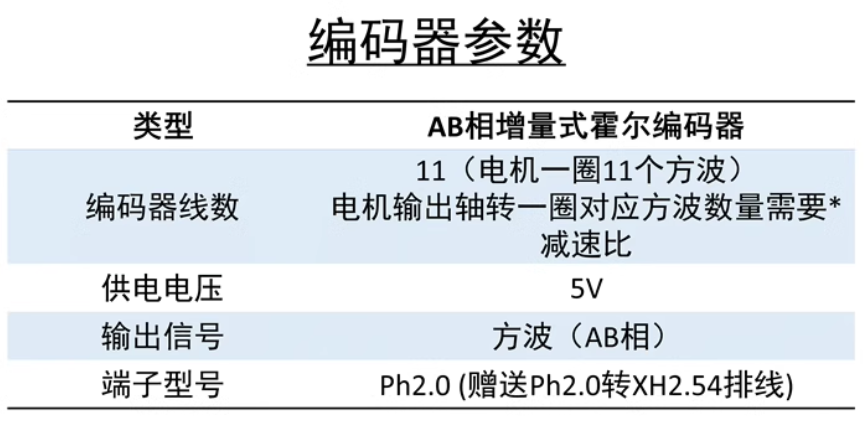
\includegraphics[width=0.6\textwidth]{motor/motor_parameter2.png}
    \caption{编码器参数图}
    \label{fig:motor_parameter2}
\end{figure}

\begin{figure}[H]
    \centering
    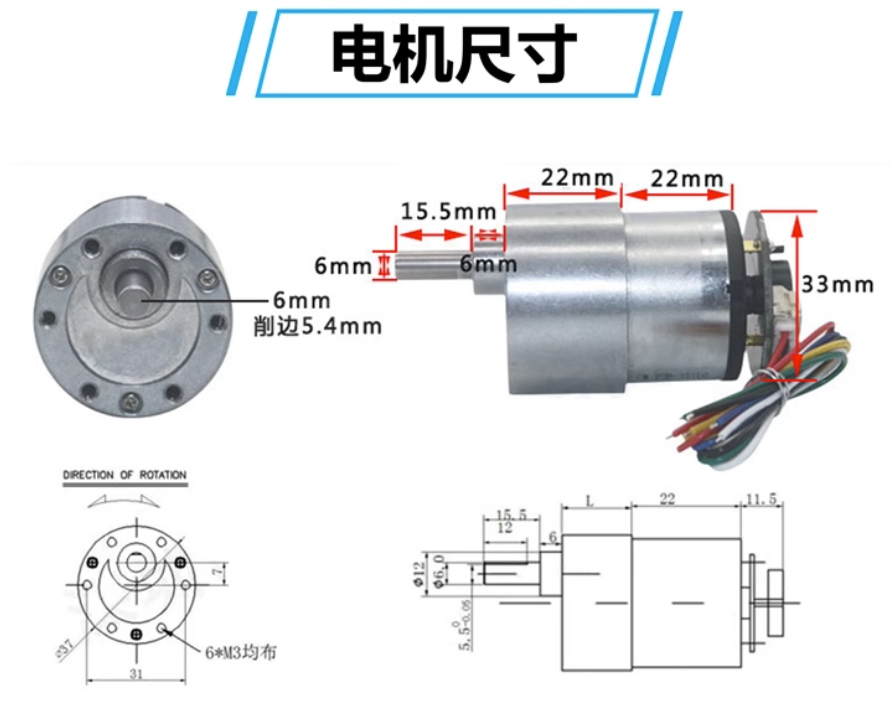
\includegraphics[width=0.6\textwidth]{motor/motor_parameter3.png}
    \caption{电机结构尺寸图}
    \label{fig:motor_parameter3}
\end{figure}

机械臂的闭合由舵机控制。根据矿石质量较轻的要求,我们选择了两个扭矩为 \SI{30}{\kilogram\cdot\centi\meter} 的舵机。舵机的额定电压范围为 \SIrange{4.8}{6.8}{\volt},线长为 \SI{30}{\centi\meter},角度范围为 \SI{180}{\degree},额定电流为 \SI{1.5}{\ampere}。


\begin{figure}[H]
    \centering
    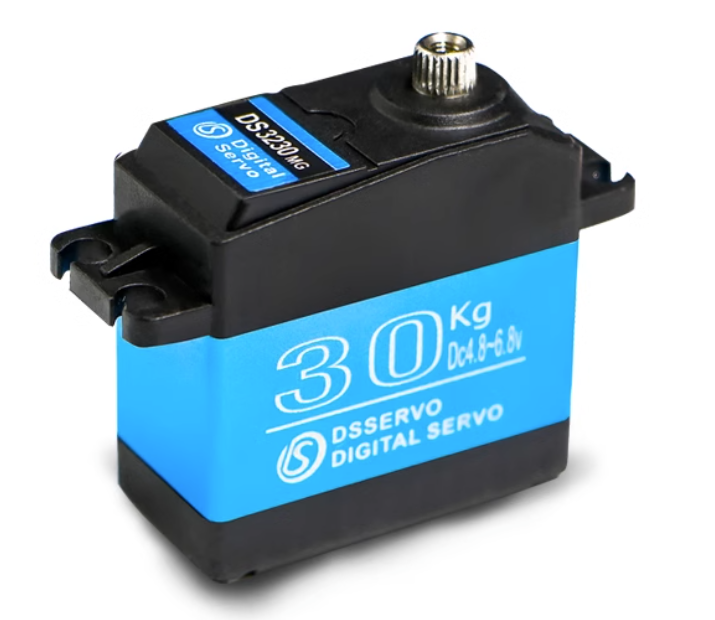
\includegraphics[width=0.5\textwidth]{motor/steer_motor.png}
    \caption{舵机}
    \label{fig:steer_motor}
\end{figure}

\begin{figure}[H]
    \centering
    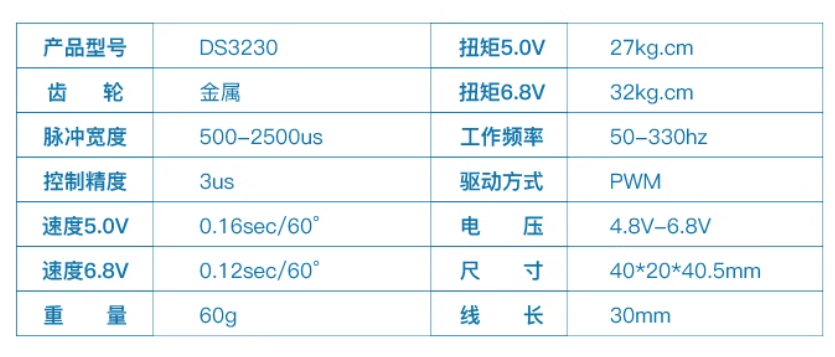
\includegraphics[width=0.8\textwidth]{motor/steer_motor_parameter.png}
    \caption{舵机参数图}
    \label{fig:steer_motor_parameter}
\end{figure}
\subsubsection{电机驱动模块}
电机驱动模块选用L298N直流电机驱动板模块。该模块的驱动电压范围为\SIrange{5}{35}{\volt}。


\begin{figure}[H]
    \centering
    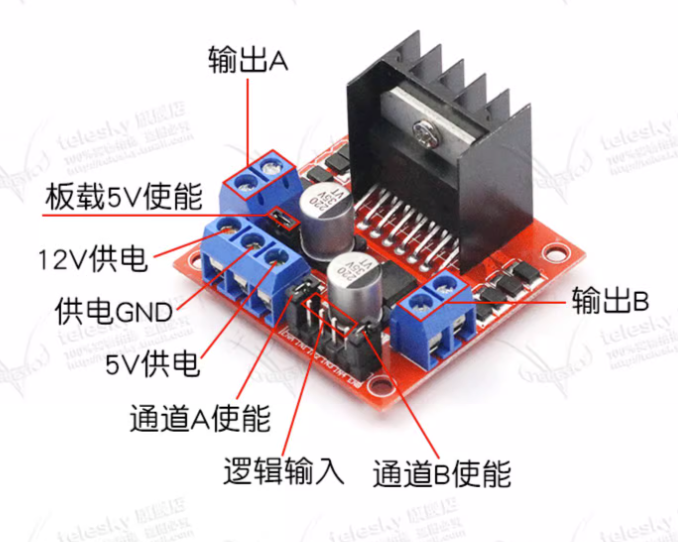
\includegraphics[width=0.6\textwidth]{drive/drive.png}
    \caption{直流电机驱动模块}
    \label{fig:drive}
\end{figure}

\begin{figure}[H]
    \centering
    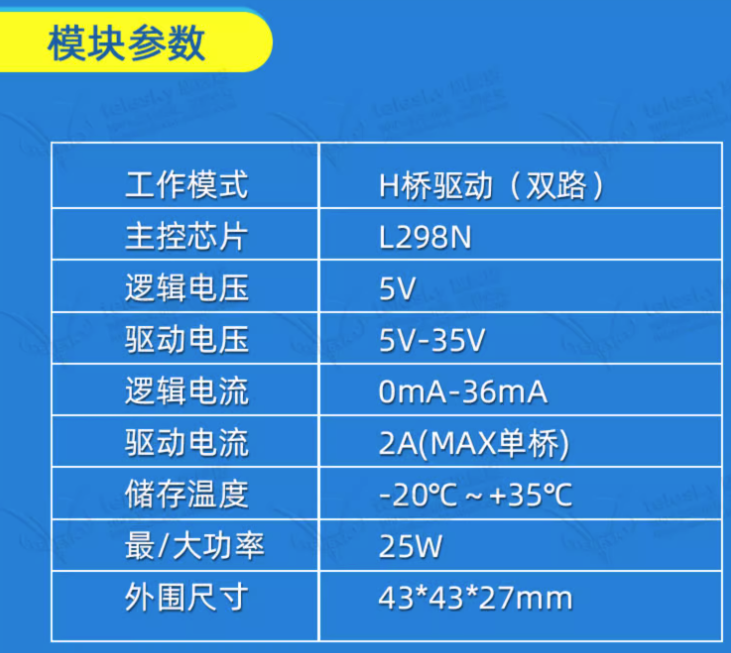
\includegraphics[width=0.6\textwidth]{drive/drive_parameter1.png}
    \caption{直流电机驱动模块参数图}
    \label{fig:drive_parameter1}
\end{figure}

\begin{figure}[H]
    \centering
    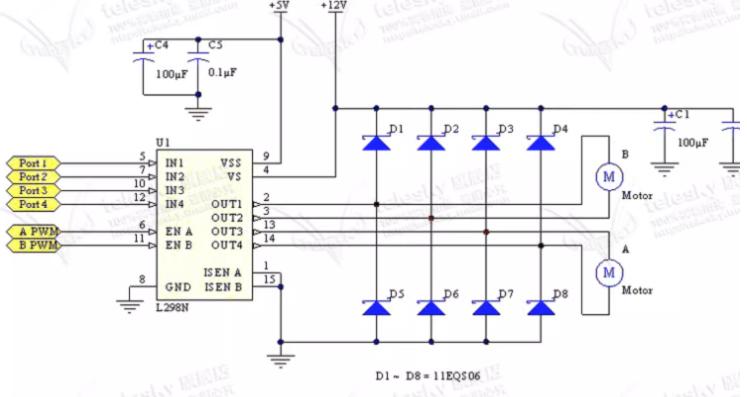
\includegraphics[width=0.6\textwidth]{drive/drive_parameter2.png}
    \caption{直流电机驱动模块电路结构图}
    \label{fig:drive_parameter2}
\end{figure}
\subsubsection{巡线模块}
巡线模块采用亚博智能小车机器人4路循迹模块巡线传感器,工作电流:\SI{0.05}{\ampere},工作电压:\SI{5}{\volt},最大探测距离:\SI{0.1}{\meter},最近探测距离:\SI{0.01}{\meter}。

\begin{figure}[H]
    \centering
    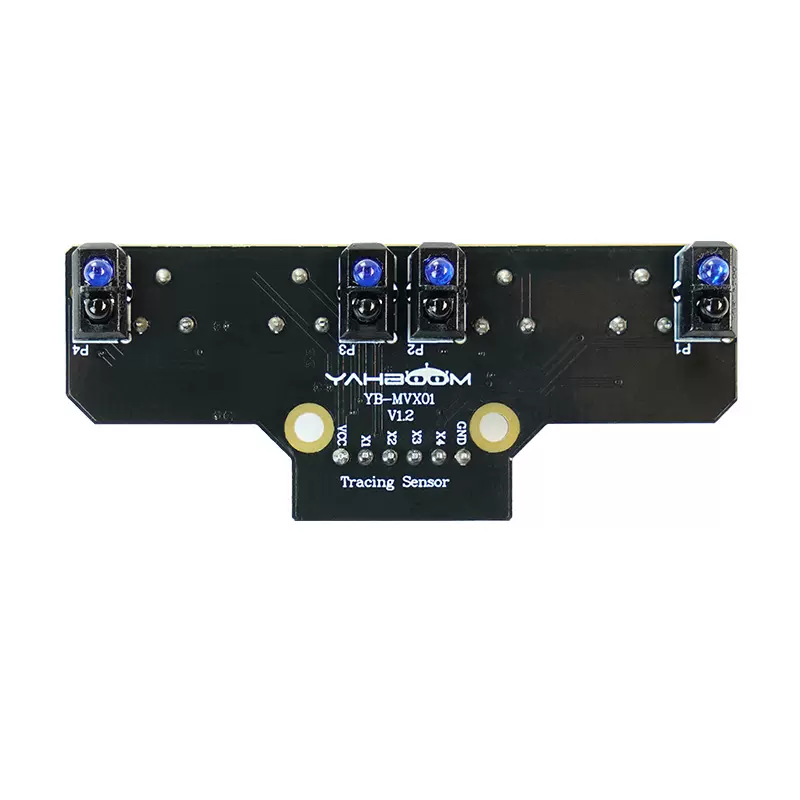
\includegraphics[width=0.6\textwidth]{patrol/patrol.png}
    \caption{巡线模块}
    \label{fig:patrol}
\end{figure}

\begin{figure}[H]
    \centering
    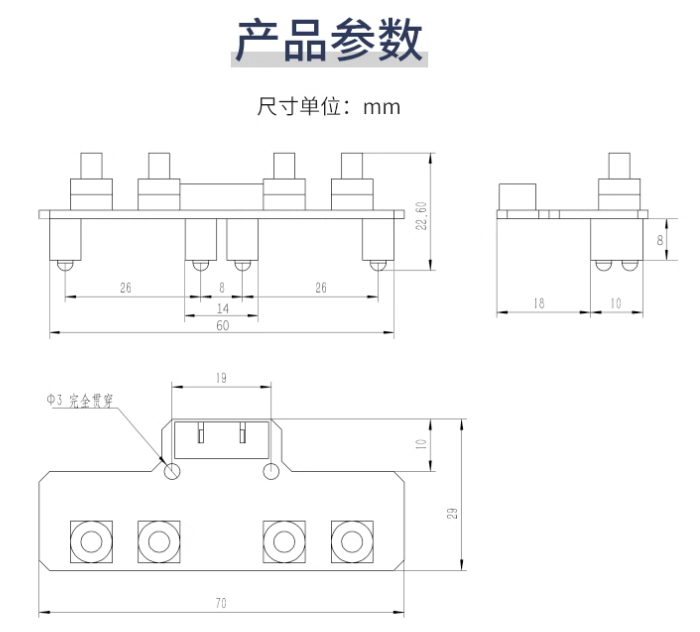
\includegraphics[width=0.6\textwidth]{patrol/patrol_parameter1.png}
    \caption{巡线模块结构尺寸图}
    \label{fig:patrol_parameter1}
\end{figure}

\begin{figure}[H]
    \centering
    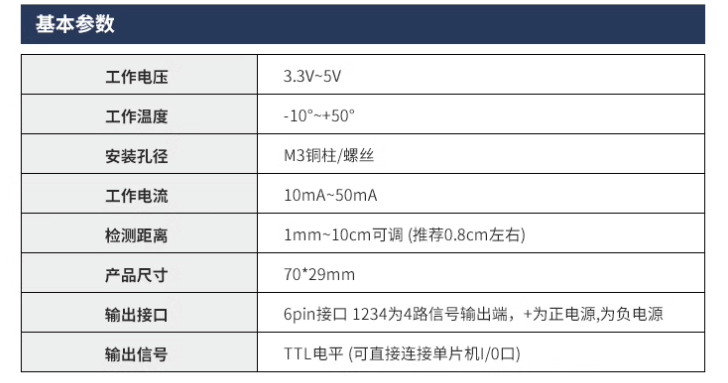
\includegraphics[width=0.6\textwidth]{patrol/patrol_parameter2.png}
    \caption{巡线模块参数图}
    \label{fig:patrol_parameter2}
\end{figure}
\clearpage


\section{算法部分}
\subsection{控制思路}

由于每次最多携带三个矿石,一共八个矿石,所以我们计划来往三轮,前两轮前往矿山采矿区,每轮采回两个富晶体矿和一个燃料矿;后一轮前往平地采矿区采矿,采回两个富晶体矿。
\subsection{主控程序设计方案}
\subsubsection{总流程}

按照控制思路,我们分三轮控制小车行为,每轮分为前往采矿区,采矿,回飞船区以及放矿这四个步骤,如图 \ref{fig:main_flow} 所示。

\begin{wrapfigure}{r}{0.3\textwidth} % 图片放置在右侧
    \centering
    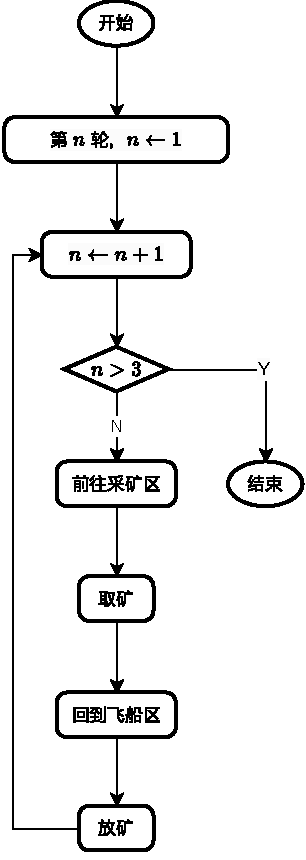
\includegraphics{algo/main_flow.pdf}
    \caption{总流程图}
    \label{fig:main_flow}
\end{wrapfigure}


\subsubsection{前往采矿区和回飞船区流程}
根据前往的矿区不同,我们分别会有不同的巡线路径前往采矿区。第一二轮我们出发后沿黑线往地图正下方走,走上陡坡后小车在第一个十字口左转,然后下一个十字口右转,进入矿山采矿区(如图中红线路径);第三轮我们出发后沿黑线往地图正右方向走,走到巡线尽头处后小车右转,然后越障前进进入平地采矿区(如图中蓝线路径)。

回飞船区同前往采矿区流程,沿前往采矿区的路线原路返回,回到出发点,如图 \ref{fig:way2} 所示。

\vfill

\begin{wrapfigure}{l}{0.7\textwidth} % 图片放置在右侧
    \centering
    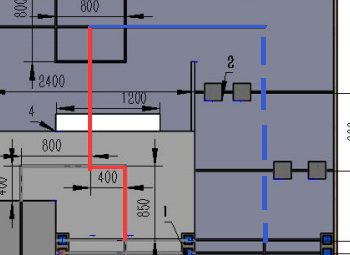
\includegraphics{algo/way2.png}
    \caption{来往路线示意图}
    \label{fig:way2}
\end{wrapfigure}
\vfill

\clearpage

\subsubsection{取矿流程}
我们通过判断当前车上的矿石数量是否足够来控制取矿流程。其中开采晶体矿时需要识别是否为富矿,开采燃料矿时需要识别是否有矿。

\begin{figure}[H]
    \centering
    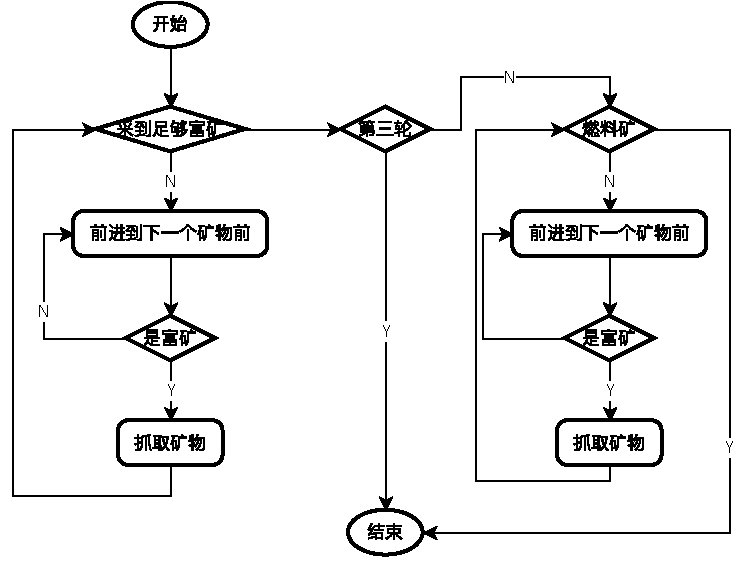
\includegraphics{algo/mining.pdf}
    \caption{取矿流程图}
    \label{fig:mining}
\end{figure}

\subsubsection{放矿流程}
此时我们已经回到了出发点,需要前往放矿区分别在对应区域内放下矿石。我们让小车分别巡线至两个货舱面前,放下矿石,然后回到出发点。巡线路径如图所示。

\begin{figure}[H]
    \centering
    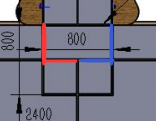
\includegraphics{algo/way_putdown.png}
    \caption{放矿路线示意图}
    \label{fig:way_putdown}
\end{figure}

\subsection{运动控制}
\subsubsection{麦克纳姆轮}
麦克纳姆轮是一种可全方位移动的全向轮,简称麦轮,由轮毂和围绕轮毂的辗子组成,麦轮混子轴线和轮毂轴线夹角成45°。在轮毂的轮缘上斜向分布着许多小轮子,即辑子,故轮子可以横向滑移。鲲子是一种没有动力的小滚子,小滚子的母线很特殊,当轮子绕着固定的轮心轴转动时,各个小滚子的包络线为圆柱面,所以该轮能够连续地向前滚动。由四个这种轮加以组合,可以使机构实现全方位移动功能。
\begin{figure}[H]
    \centering
    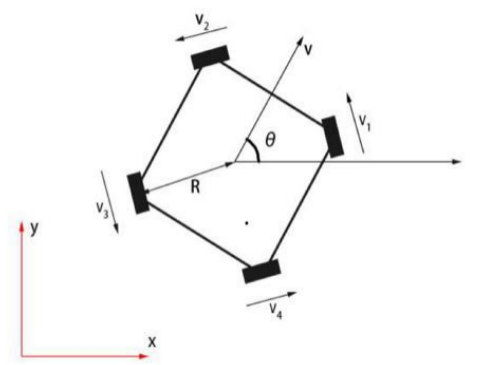
\includegraphics{algo/Mwheel.png}
    \caption{麦克纳姆轮速度合成分解示意图}
    \label{fig:Mwheel}
\end{figure}
四个轮子转动时,会产生四个方向的速度和动力,我们将其分解合成就可以得到小车在两坐标轴上的速度以及小车自身的角速度。这个过程等价于解一个矩阵方程。

\begin{equation*}
    \begin{pmatrix}
        v_1 \\v_2\\v_3\\v_4
    \end{pmatrix}
    =
    \begin{pmatrix}
        -\sin \phi & \cos \phi  & R \\
        -\cos \phi & -\sin \phi & R \\
        \sin \phi  & -\cos \phi & R \\
        \cos \phi  & \sin \phi  & R
    \end{pmatrix}
    \begin{pmatrix}
        v_x \\v_y\\ w
    \end{pmatrix}
\end{equation*}
其中,$\theta$ 为小车速度方向与 $x$ 轴夹角,$\phi= \theta - 45\si{\degree}$;$w$ 是小车的角速度,取逆时针为正方向;$R$ 是小车底盘中心到轮子中心的距离。

\subsubsection{红外巡线}
我们选择一个红外巡线装置来巡线和控制小车,一个红外巡线足以保证小车自身行驶在黑线上,也能保证走到十字路口时能够检测到。

本次比赛起巡线作用的是三路巡线模块,采用模拟量输入(\SIrange{0}{1023}{}) 。通过实验得到三个红外管在检测到黑线时的阈值,用来判断传感器是否在黑线内;若不完全在黑线内,可以比较两侧红外管的模拟量输入,来判断传感器相对黑线位置,通过单片机控制电机直到三个红外管模拟量均在阈值之内。

\subsection{驱动控制}
\subsubsection{直流有刷电机}
直流有刷电机用于驱动小车,我们采用PWM来控制电机。PWM 指的是脉冲宽度调制,其本质是一种数字信号,主要由两个组成部分来进行定义,分别是占空比和频率,其中占空比值得是信号为高电平状态的时间量占据总周期时间的百分比,而频率则代表着 PWM 信号完成一个周期的速度,也就是决定信号在高低电平状态之间的切换速度。占空比越大,代表高电平状态所占的比例越大,也就是电机的速度会越快。当信号在高低电平之间切换的较快时,电机的速度就可以保持在一个平稳的水平上,这也就达到了控制转速的目的。
\begin{figure}[H]
    \centering
    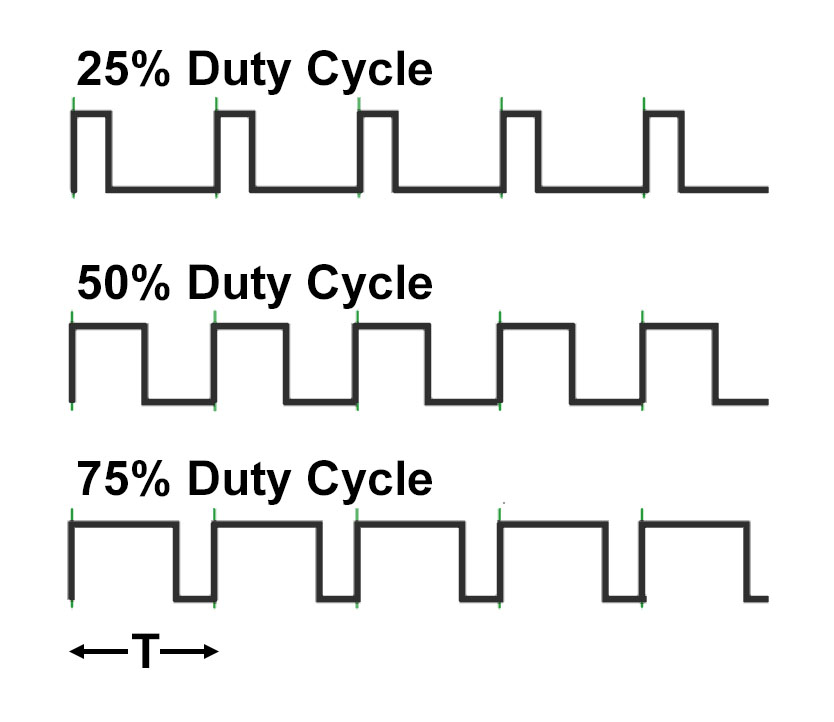
\includegraphics[width = 0.4\textwidth]{algo/PWM.jpg}
    \caption{PWM控制直流有刷电机}
    \label{fig:dianji}
\end{figure}
\subsubsection{舵机}
舵机用在机器臂的伸缩和矿石的抓取,我们同样采用PWM来控制。舵机首先接收PWM 信号,当信号进入内部电路产生一个偏置电压,触发电机通过减速齿轮带动电位器移动,使电压差为零时,电机停转,从而达到伺服的效果。简单来说就是给舵机一个特定的 PWM 信号,舵机就可以旋转到指定的位置。
\begin{figure}[H]
    \centering
    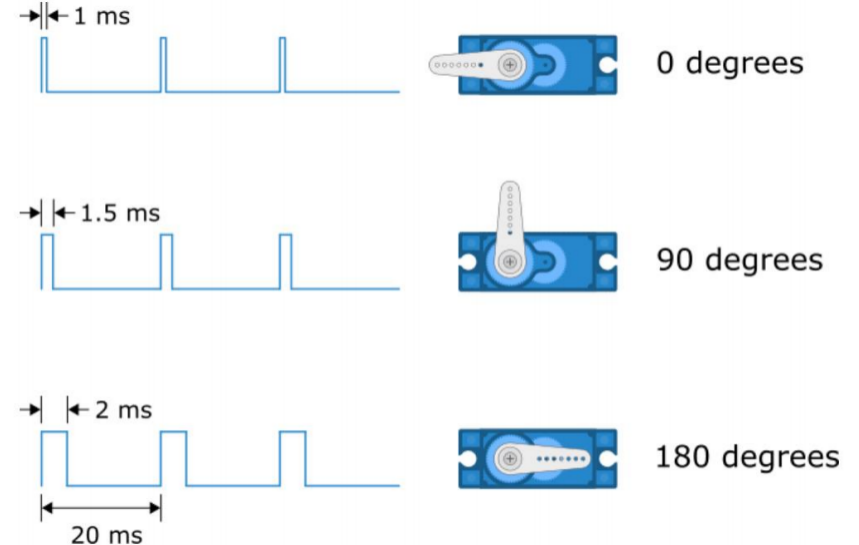
\includegraphics[width = 0.6\textwidth]{algo/duoji.png}
    \caption{PWM控制舵机}
    \label{fig:duoji}
\end{figure}
\subsection{PID控制算法}

PID控制,或者称之为比例-积分-微分控制,结合了三种反馈控制方式:比例控制,积分控制以及微分控制。其可以根据控制对象和应用条件,采用这三种控制方式的部分组合,如P控制,PI控制,PD控制或者是三者的组合,即真正意义上的PID控制。整体上,我们将这些称为PID控制律,而采用这种控制规律的控制器被称为PID控制器。

\vfill
\begin{figure}[H]
    \centering
    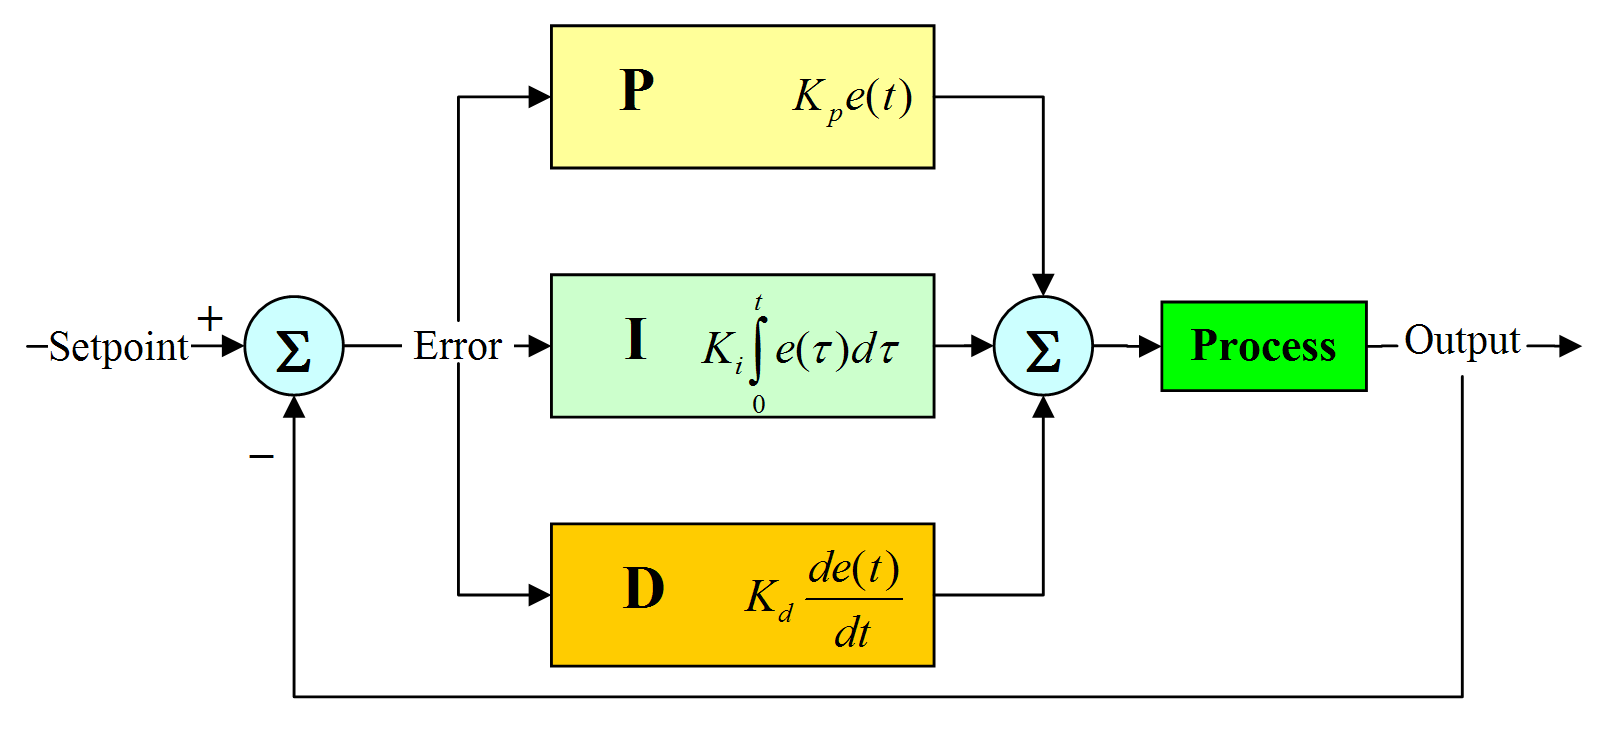
\includegraphics[width = 0.8\textwidth]{algo/PID.png}
    \caption{PID控制算法}
    \label{fig:PID}
\end{figure}

PID控制器的控制公式可以表示为:
\begin{equation*}
    u(t) = K_p e(t) + K_i \int_0^t e(\tau) \mathrm{~d}\tau + K_d \frac{\mathrm{d} e(t)}{\mathrm{d}t}
\end{equation*}
其中:

\begin{itemize}
    \item $u(t)$ 是控制器的输出
    \item $K_p$ 是比例增益,是一个调适参数
    \item $K_i$ 是积分增益,也是调适参数
    \item $K_d$ 是微分增益,也是调适参数
    \item $e(t)$ 是误差,定义为设定值(SP)减去回授值(PV)
    \item $t$ 是当前时间
\end{itemize}


以下是对这三个增益的更详细解释:

\begin{enumerate}[label = \arabic{*}.]
    \item 比例增益$K_p$:比例控制考虑当前的误差,误差值和一个正值的常数$K_p$(表示比例)相乘。需要控制的量,比如水温,有它现在的当前值,也有我们期望的目标值。实际编程时,就让偏差(目标减去当前)与调节装置的“调节力度”,建立一个一次函数的关系,就可以实现最基本的“比例”控制了。$K_p$越大,调节作用越激进,$K_p$调小会让调节作用更保守。
    \item 微分增益$K_d$:微分控制考虑将来的误差,计算误差的一阶导,并和一个正值的常数$K_d$相乘。$K_d$的作用就是让物理量的速度趋于0,只要什么时候,这个量具有了速度,$K_d$就向相反的方向用力,尽力刹住这个变化。$K_d$参数越大,向速度相反方向刹车的力道就越强。
    \item 积分增益$K_i$:积分控制考虑过去的误差,将过去一段时间的误差和乘以一个正值的常数$K_i$。$K_i$的值越大,积分时乘的系数就越大,积分效果越明显,所以,$K_i$的作用就是,减小静态情况下的误差,让受控物理量尽可能接近目标值。在使用积分控制时,需要设定积分限制,防止在初始状态时,就把积分量积得太大,难以控制。
\end{enumerate}

% 调试PID算法的参数,即通过调整控制参数(比例增益,积分增益,微分增益)让系统达到最佳的控制效果,是实现PID控制的关键一步。在调试过程中,确保系统的稳定性(即不会发生发散性的震荡)是首要条件。然而,不同的系统可能会有不同的行为,不同的应用其需求也可能会不同,而且这些需求还可能会相互冲突。因此,PID控制参数的调试是一项充满挑战的任务。

% 总的来说,PID控制是一种强大而灵活的控制算法,可以适用于许多不同类型的系统和应用。通过适当地调整比例,积分和微分增益,可以实现对系统的精确控制,从而达到预期的性能和响应。



\subsection{视觉方案}
\subsubsection{概述}
本次比赛在抓取矿物、判断富矿和避障时需要使用到图像处理操作。
\begin{itemize}
    \item 抓取矿物:使用边缘检测算法,例如Canny算法,可以帮助确定矿物的轮廓。这可以通过将矿物与其背景区分开来,从而确定其位置和形状。然后,这些信息可以用来指导机器人的抓取器进行精确的抓取。
    \item 判断富矿:颜色识别是一种常见的图像处理技术,可以用于判断矿物的颜色。可以通过对图像进行颜色空间转换(如RGB到HSV)以及阈值处理,来识别出图像中的特定颜色(在这里是橘色)。然后,这个信息可以用来判断哪些矿物是富矿。
    \item 避障:同样地,边缘检测也可以用来检测出图像中的障碍物。通过找到障碍物的边缘,可以确定其位置和形状,从而计算出安全的路径,避免机器人碰到障碍物。
\end{itemize}

\subsubsection{边缘检测算法}

Canny边缘检测算法是一种非常流行和广泛应用的边缘检测方法,与其他一些常见的边缘检测算法相比,Canny边缘检测算法有以下优点:

\begin{enumerate}
    \item 低误报率:Canny边缘检测对图像进行了平滑处理,以减少由噪声引起的错误检测。然后,通过使用双阈值检测和边缘连接,Canny进一步消除了不连续和假边缘,从而减少了误报。
    \item 定位精度:由于Canny算法在进行非极大值抑制步骤时,会沿着梯度方向检查像素点,这样可以精确地定位到边缘的位置,保证边缘定位的精度。
    \item 响应单一:Canny边缘检测算法的另一个目标是只对边缘响应一次,并且尽可能地将响应定位到边缘的中心。非极大值抑制步骤就是为了实现这一目标。
    \item 能检测到弱边缘:通过双阈值检测和边缘连接,Canny能够链接断开的边缘,检测到由于噪声或者色彩变化而形成的弱边缘。
\end{enumerate}

这些优点使得Canny边缘检测算法在许多应用中成为首选的边缘检测方法,尤其是在需要高精度边缘检测的场合,如机器视觉和医疗图像分析等。

\begin{enumerate}
    \item 使用高斯滤波器对图像进行平滑处理以消除噪声。
    \item 计算图像的梯度强度和方向。
    \item 应用非极大值抑制(Non-Maximum Suppression)以消除边缘响应的宽度。
    \item 使用双阈值(Double Threshold)确定边缘。
    \item 通过抑制孤立的低阈值像素最终确定边缘。
\end{enumerate}

下面是Canny边缘检测算法的一个简单的伪代码表示:

\begin{center}
    \begin{minipage}{0.7\textwidth}
        \begin{algorithm}[H]
            \SetAlgoLined
            \KwResult{Edge Image}
            \textbf{Input:} {image}

            smoothedImage = GaussianBlur(image)\;
            gradientImage, gradientDirection = ComputeGradient(smoothedImage)\;
            nmsImage = NonMaximumSuppression(gradientImage, gradientDirection)\;
            doubleThresholdImage = DoubleThreshold(nmsImage)\;
            edgeImage = SuppressIsolatedPixels(doubleThresholdImage)\;
            \Return{edgeImage}\;

            \caption{Canny Edge Detection Algorithm}
        \end{algorithm}
    \end{minipage}
\end{center}




\subsubsection{HSV色彩空间}
HSV色彩空间是一种由Hue(色调)、Saturation(饱和度)和Value(明度)三个分量构成的颜色空间。HSV色彩空间与RGB色彩空间的主要区别在于它更接近人类对颜色的感知方式。
\begin{figure}[H]
    \centering
    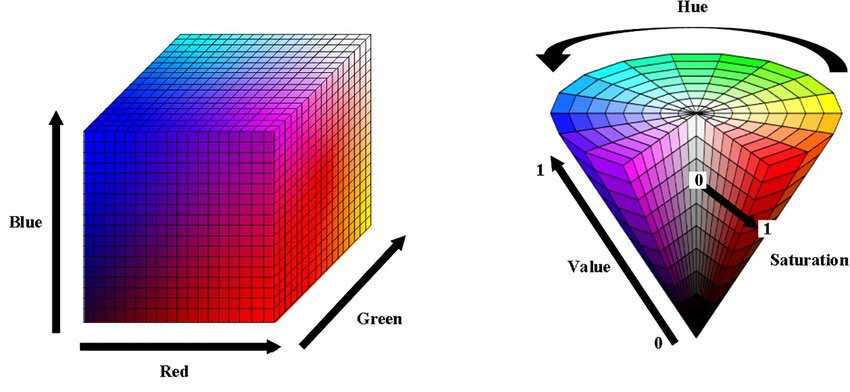
\includegraphics[width = 0.8\textwidth]{algo/RGB_HSV.jpg}
    \caption{RGB和HSV色彩空间}
    \label{fig:HSV}
\end{figure}

\begin{itemize}
    \item Hue(色调):表示颜色的种类,例如红色、蓝色等。
    \item Saturation(饱和度):表示颜色的强烈程度或纯度。饱和度低的颜色接近灰色,饱和度高的颜色则看起来更鲜艳。
    \item Value(明度):表示颜色的明亮程度。低明度的颜色看起来更暗,高明度的颜色看起来更亮。
\end{itemize}

在视觉处理上,HSV色彩空间具有一些优势。RGB色彩空间中,三种颜色通道(红、绿、蓝)是均匀混合的,这与人类的颜色感知不完全一致。相比之下,HSV色彩空间将颜色的属性分离开来,更符合人类对颜色的感知方式。



\clearpage
\section{经费预算}
\begin{table}[H]
    \centering
    \caption{经费预算}
    \begin{tabular}{cccrr}
        \toprule
        类别                  & 项目               & 数量 & 预计单价   & 预计总价              \\
        \midrule
        \multirow{5}{*}{机械} & 板材及管材            & 若干 & -      & 300.00            \\
                            & 麦克纳姆轮            & 4  & 125.00 & 500.00            \\
                            & 胶轮               & 4  & 50.00  & 200.00            \\
                            & 机械臂及机械爪所需零部件     & 若干 & -      & 800.00            \\
                            & 深沟球轴承            & 1  & 200.00 & 200.00            \\
        \hline
        \multirow{8}{*}{电控} & 锂电池2600mAh       & 4  & 69.80  & 279.20            \\
                            & 锂电池10400mAh      & 1  & 229.80 & 229.80            \\
                            & 降压模块5A           & 4  & 26.06  & 104.24            \\
                            & STM32F407ZGT6系统板 & 2  & 402.32 & 804.64            \\
                            & 树莓派4B            & 1  & 849.00 & 849.00            \\
                            & 直流减速电机           & 4  & 70.00  & 280.00            \\
                            & 单轴舵机             & 4  & 150.00 & 600.00            \\
                            & 电机驱动模块L298N      & 4  & 19.30  & 77.20             \\
        \hline
        \multirow{2}{*}{算法} & 巡线模块             & 4  & 29.80  & 119.20            \\
                            & 摄像头              & 1  & 150.00 & 150.00            \\
        \hline
        合计                  &                  &    &        & 约\textyen 5500.00 \\
        \bottomrule
    \end{tabular}
    \label{tab:budget}
\end{table}


\clearpage
\section{时间安排}

\begin{table}[H]
    \centering
    \caption{时间安排}
    \begin{tabular}{cl}
        \toprule
        时间                                   & {\centering 进度}             \\
        \midrule
        5月7日                                 & 确定组员,预报名                    \\
        5月11日                                & 第一次会议,确定分工,开始计划书撰写          \\
        5月26日                                & 第二次会议,进展汇报,开始计划书完善修改        \\
        6月4日                                 & 计划书提交                       \\
        6月5日 ~ 7月28日(一审)                     & 参加培训,深入学习各自负责模块的知识,采购、加工零件  \\
        8月1日 ~ 8月31日(二审)                     & 完成机械结构的安装与调试, 能够初步实现比赛动作    \\
        \multirow{2}[0]{*}{9月1日 ~ 9月28日(三审)} & 完成电路布置,测试控制程序,调整优化部分机械结构设计, \\
                                             & 机器人能够基本完成所有比赛动作             \\
        9月29日 ~ 10月13日(预选赛)                  & 优化控制程序,完善代码,机器人能够流畅实现比赛全过程  \\
        10月14日(决赛)                           & 进一步优化及完善,提高速度,在场地调试         \\
        \bottomrule
    \end{tabular}
    \label{tab:timeline}
\end{table}




\end{document}
